\documentclass[10pt,article,oneside]{memoir}
\usepackage[top=1.2in, bottom=1.2in, left=1.4in, right=1.4in]{geometry}

\usepackage{amssymb, amsmath, amsthm, mathtools}

% Essential packages
\usepackage{color}
\usepackage{graphicx}
\usepackage{tabularx}
\usepackage{longtable}
\usepackage{enumitem}
\usepackage{url}
\usepackage{float}


% Colors ------------
\usepackage{xcolor}
\definecolor{mygray}{gray}{0.5} % define color on gray scale
\definecolor{lgray}{gray}{0.9} % define color on gray scale
\definecolor{crimson}{RGB}{153,0,0}
\definecolor{dgray}{RGB}{125,125,125}
\newcommand{\crimson}[1]{\textcolor{crimson}{#1}}
  \newcommand{\dgray}[1]{\textcolor{dgray}{#1}}
    \newcommand{\lgray}[1]{\textcolor{lgray}{#1}}
      \newcommand{\mygray}[1]{\textcolor{mygray}{#1}}

% Hyperref
\usepackage[pdfencoding = auto, 
            hidelinks = true, 
            urlcolor = crimson, 
            linkcolor = black,
            colorlinks = true]{hyperref}


% Parameters
\usepackage{soul} % underline

% Minion for main text and math
% \usepackage{MinionPro}

% Helvetica for sans serif
% (scaled to match size of Minion)
\usepackage[scaled=0.95]{helvet}

% Bera Mono for monospaced
% (scaled to match size of Minion)
\usepackage[T1]{fontenc}
\usepackage[scaled=0.9]{beramono}
% \usepackage{fontspec}
% \setmonofont[Scale=0.85]{Monaco}

% FORCE HELVET
\renewcommand\familydefault{\sfdefault}

% Spacing
\usepackage{setspace}

% Sectioing
\setcounter{secnumdepth}{0} % fix starting with "0.1"
\usepackage{titlesec}
\titleformat*{\section}{\Huge\bfseries}

% Dash 
\renewcommand\labelitemi{--}

% Theorems
\usepackage{etoolbox}
\renewcommand{\qedsymbol}{\rule{0.7em}{0.7em}}
\newtheorem{theorem}{Theorem}
\newtheorem{lem}{Lemma}
\newtheorem{assump}{Assumption}
\theoremstyle{definition}
\newtheorem{definition}{Definition}
\AtEndEnvironment{definition}{\null\hfill\qedsymbol}%
\newtheorem{example}{Example}
\newtheorem{error}{Common Error}
\AtEndEnvironment{error}{\null\hfill\qedsymbol}%

% Math
\newcommand{\var}{\textnormal{Var}}
\newcommand{\cov}{\textnormal{Cov}} 
\newcommand{\cor}{\textnormal{Cor}} 

% Figures
\usepackage{graphicx,grffile}
\makeatletter
\def\maxwidth{\ifdim\Gin@nat@width>\linewidth\linewidth\else\Gin@nat@width\fi}
\def\maxheight{\ifdim\Gin@nat@height>\textheight\textheight\else\Gin@nat@height\fi}
\makeatother

% Scale images if necessary, so that they will not overflow the page
% margins by default, and it is still possible to overwrite the defaults
% using explicit options in \includegraphics[width, height, ...]{}
\setkeys{Gin}{width=\maxwidth,height=\maxheight,keepaspectratio}


% SVG
% \usepackage{svg}


% Shading and Rmd macros
\usepackage{color}
\usepackage{fancyvrb}
\newcommand{\VerbBar}{|}
\newcommand{\VERB}{\Verb[commandchars=\\\{\}]}
\DefineVerbatimEnvironment{Highlighting}{Verbatim}{commandchars=\\\{\}}
% Add ',fontsize=\small' for more characters per line
\usepackage{framed}
\definecolor{shadecolor}{RGB}{248,248,248}
\newenvironment{Shaded}{\begin{snugshade}}{\end{snugshade}}
\newcommand{\AlertTok}[1]{\textcolor[rgb]{0.94,0.16,0.16}{#1}}
\newcommand{\AnnotationTok}[1]{\textcolor[rgb]{0.56,0.35,0.01}{\textbf{\textit{#1}}}}
\newcommand{\AttributeTok}[1]{\textcolor[rgb]{0.77,0.63,0.00}{#1}}
\newcommand{\BaseNTok}[1]{\textcolor[rgb]{0.00,0.00,0.81}{#1}}
\newcommand{\BuiltInTok}[1]{#1}
\newcommand{\CharTok}[1]{\textcolor[rgb]{0.31,0.60,0.02}{#1}}
\newcommand{\CommentTok}[1]{\textcolor[rgb]{0.56,0.35,0.01}{\textit{#1}}}
\newcommand{\CommentVarTok}[1]{\textcolor[rgb]{0.56,0.35,0.01}{\textbf{\textit{#1}}}}
\newcommand{\ConstantTok}[1]{\textcolor[rgb]{0.00,0.00,0.00}{#1}}
\newcommand{\ControlFlowTok}[1]{\textcolor[rgb]{0.13,0.29,0.53}{\textbf{#1}}}
\newcommand{\DataTypeTok}[1]{\textcolor[rgb]{0.13,0.29,0.53}{#1}}
\newcommand{\DecValTok}[1]{\textcolor[rgb]{0.00,0.00,0.81}{#1}}
\newcommand{\DocumentationTok}[1]{\textcolor[rgb]{0.56,0.35,0.01}{\textbf{\textit{#1}}}}
\newcommand{\ErrorTok}[1]{\textcolor[rgb]{0.64,0.00,0.00}{\textbf{#1}}}
\newcommand{\ExtensionTok}[1]{#1}
\newcommand{\FloatTok}[1]{\textcolor[rgb]{0.00,0.00,0.81}{#1}}
\newcommand{\FunctionTok}[1]{\textcolor[rgb]{0.00,0.00,0.00}{#1}}
\newcommand{\ImportTok}[1]{#1}
\newcommand{\InformationTok}[1]{\textcolor[rgb]{0.56,0.35,0.01}{\textbf{\textit{#1}}}}
\newcommand{\KeywordTok}[1]{\textcolor[rgb]{0.13,0.29,0.53}{\textbf{#1}}}
\newcommand{\NormalTok}[1]{#1}
\newcommand{\OperatorTok}[1]{\textcolor[rgb]{0.81,0.36,0.00}{\textbf{#1}}}
\newcommand{\OtherTok}[1]{\textcolor[rgb]{0.56,0.35,0.01}{#1}}
\newcommand{\PreprocessorTok}[1]{\textcolor[rgb]{0.56,0.35,0.01}{\textit{#1}}}
\newcommand{\RegionMarkerTok}[1]{#1}
\newcommand{\SpecialCharTok}[1]{\textcolor[rgb]{0.00,0.00,0.00}{#1}}
\newcommand{\SpecialStringTok}[1]{\textcolor[rgb]{0.31,0.60,0.02}{#1}}
\newcommand{\StringTok}[1]{\textcolor[rgb]{0.31,0.60,0.02}{#1}}
\newcommand{\VariableTok}[1]{\textcolor[rgb]{0.00,0.00,0.00}{#1}}
\newcommand{\VerbatimStringTok}[1]{\textcolor[rgb]{0.31,0.60,0.02}{#1}}
\newcommand{\WarningTok}[1]{\textcolor[rgb]{0.56,0.35,0.01}{\textbf{\textit{#1}}}}


% Parmaters

\title{ \LARGE\textbf{Guide to the CCES Cumulative Common Content (2006
- 2021)}}
 

\author{\href{https://orcid.org/0000-0002-5687-2647}{\XeTeXLinkBox{\raisebox{-0.1em}{
\includegraphics[width=1em]{orcid.png}}}}~Shiro
Kuriwaki\thanks{Department of Political Science, Yale University.
Website: \url{https://www.shirokuriwaki.com}. ORCID:
\url{https://orcid.org/0000-0002-5687-2647}. My thanks to Alexander
Agadjanian, Steve Ansolabehere, Stephen DiMauro, Bernard Fraga, Nathan
Kaplan, Silvia Kim, Mayya Komisarchik, Stephen Pettigrew, Boris Shor,
Brian Schaffner, and Gerlad Wright for their suggestions and
contributions. Thanks to Joe Williams at YouGov, and Jon Keane, Mike
Malecki, and Gordon Shotwell at Crunch for their help.}}


\date{Guide last updated: 2022-03-23}

\begin{document}

\maketitle





\renewcommand\UrlFont{\color{crimson}\ttfamily}

\noindent \emph{Cite this dataset as:}

\begin{quote}
Kuriwaki, Shiro, 2022, ``Cumulative CCES Common Content'',
\href{https://dataverse.harvard.edu/dataset.xhtml?persistentId=doi:10.7910/DVN/II2DB6}{\url{doi:10.7910/DVN/II2DB6}},
Harvard Dataverse, V7.
\end{quote}

\bigskip

This dataset combines 16 years (2006 -- 2021) of the Cooperative
Congressional Election Study (CCES), renamed the Cooperative
Congressional Election Study (CES) from 2020. The CCES/CES is an online
survey conducted around November of each year, asking a range of
questions on political behavior and public opinion. Its principal
investigators are Stephen Ansolabehere, Sam Luks, and Brian Schaffner.

\bigskip

Each year's CCES/CES asks hundreds of questions, many of which change
from year to year. This cumulative file only includes \emph{a subset} of
those questions that are standard and important. It standardizes
(harmonizes) its values across years and creates a few new variables
too. Users can still merge in their year-specific questions of interest
easily into this cumulative file and take advantage of its standardized
variables.

\bigskip

I constructed this dataset from each year's full CCES/CES, all of them
publicly available as separate datasets on
\href{cces.gov.harvard.edu}{Dataverse}.The final product is a
\texttt{tibble}-style data frame (built in R) that is also available as
a Stata \texttt{dta} file. In addition, the same dataset is available on
\texttt{Crunch}, an analytics interface optimized for survey datasets.
The source code is open-source.

\bigskip

Please note that this cumulative dataset makes some modifications to the
original CCES/CES datasets to maintain comparability across years. These
modifications are only made when differences are deemed sufficiently
minor. Still, for details on the survey methodology and a list of all
questions, readers should consult the guides for each year.

\bigskip

\noindent\makebox[\textwidth][c]{%
\begin{minipage}{0.92\linewidth}
\begin{itemize}

\item \textbf{To see the source code, } report a bug, or ask a question about the data, please feel free to file an issue from the \href{https://github.com/kuriwaki/cces_cumulative}{source code repository}. Alternatively, please contact me by email.

\item \textbf{To obtain the individual year's CCES/CES datasets, } search the \href{https://dataverse.harvard.edu/dataverse/cces}{CES dataverse} or access the \href{https://cces.gov.harvard.edu/}{CES homepage}. Sign-up to the Crunch dataset from the homepage as well.

\item \textbf{To understand the survey methodology, } consult the \href{https://cces.gov.harvard.edu/frequently-asked-questions}{Frequently Asked Questions} page of the CES homepage or the methodology section of a \href{https://doi.org/10.7910/DVN/E9N6PH}{recent Common Content's} codebook.
\end{itemize}
\end{minipage}
}

\vspace{1cm}

\newpage
\setcounter{tocdepth}{3}
\tableofcontents*
\newpage

\hypertarget{getting-started}{%
\section{Getting Started}\label{getting-started}}

\hypertarget{data-read-in}{%
\subsection{Data Read-in}\label{data-read-in}}

The \texttt{.Rds} format can be read into R. This format preserves
dataset properties such as the distinction between integers and doubles,
and labelled variables.

\begin{Shaded}
\begin{Highlighting}[]
\NormalTok{cc }\OtherTok{\textless{}{-}} \FunctionTok{readRDS}\NormalTok{(}\StringTok{"cumulative\_2006{-}2021.Rds"}\NormalTok{)}
\end{Highlighting}
\end{Shaded}

\noindent The dataset in R is best viewed with \texttt{dplyr}, although
it can also be used without tidyverse.

\begin{Shaded}
\begin{Highlighting}[]
\FunctionTok{library}\NormalTok{(tidyverse)}
\NormalTok{cc}
\end{Highlighting}
\end{Shaded}

\noindent  A Stata dta version is provided as well.
\texttt{cumulative\_2006-2021.dta} can be read by Stata, or in R by the
\texttt{haven} package

\begin{Shaded}
\begin{Highlighting}[]
\FunctionTok{library}\NormalTok{(haven)}
\NormalTok{cc }\OtherTok{\textless{}{-}} \FunctionTok{read\_dta}\NormalTok{(}\StringTok{"cumulative\_2006{-}2021.dta"}\NormalTok{)}
\end{Highlighting}
\end{Shaded}

R is free software and, if necessary, the \texttt{haven} and
\texttt{readr} package can be used to export the CCES/CES datasets in
other formats such as plain-text csv or SPSS sav files. Plain-text
formats are somewhat less convenient because they do not preserve value
labels.

\hypertarget{data-download}{%
\subsection{Data Download}\label{data-download}}

\noindent \emph{Downloading the data via R.} In some cases, it may be
convenient to download the dataset directly into an R environment
without downloading the file to one's computer. The recent version of
\texttt{dataverse} (version 0.3.0 or later) allows this by the function:

\begin{Shaded}
\begin{Highlighting}[]
\FunctionTok{library}\NormalTok{(dataverse)}
\NormalTok{cc }\OtherTok{\textless{}{-}} \FunctionTok{get\_dataframe\_by\_name}\NormalTok{(}
  \AttributeTok{filename =} \StringTok{"cumulative\_2006{-}2021.dta"}\NormalTok{,}
  \AttributeTok{dataset =} \StringTok{"10.7910/DVN/II2DB6"}\NormalTok{,}
  \AttributeTok{original =} \ConstantTok{TRUE}\NormalTok{,}
  \AttributeTok{.f =}\NormalTok{ haven}\SpecialCharTok{::}\NormalTok{read\_dta,}
  \AttributeTok{server =} \StringTok{"dataverse.harvard.edu"}
\NormalTok{)}
\end{Highlighting}
\end{Shaded}

\hypertarget{unique-identifiers-and-how-to-add-more-variables}{%
\subsection{Unique identifiers and how to add more
variables}\label{unique-identifiers-and-how-to-add-more-variables}}

The cumulative dataset only uses key variables from each year's common
content. But users can still merge in other common content variables, or
variables from other CCES datasets like the policy preferences
dataset\footnote{Dagonel, Angelo, 2021, ``Cumulative CCES Policy Preferences'', \href{https://dataverse.harvard.edu/dataset.xhtml?persistentId=doi:10.7910/DVN/OSXDQO}{\url{doi:10.7910/DVN/OSXDQO}}, Harvard Dataverse.}.

In R, we recommend using the \texttt{left\_join} or \texttt{inner\_join}
functions (or the base-R \texttt{merge} function). In Stata, use
\texttt{merge\ 1:1}. In all cases, the combination of \texttt{year} and
\texttt{case\_id} \textbf{uniquely identifies each row} in the
cumulative common content, so any merges should merge on year and the
case identifier. For example, suppose we have separately downloaded the
\href{https://doi.org/10.7910/DVN/GDF6Z0/JPMOZZ}{2016 Common Content}
and read it in as follows:

\begin{Shaded}
\begin{Highlighting}[]
\NormalTok{cc16 }\OtherTok{\textless{}{-}} \FunctionTok{read\_dta}\NormalTok{(}\StringTok{"CCES16\_Common\_OUTPUT\_Feb2018\_VV.dta"}\NormalTok{)}
\end{Highlighting}
\end{Shaded}

Suppose we want to merge in the 2016-specific issue questions that ask
respondent's views about key votes in Congress. This variable all start
with \texttt{"CC16\_351"} and the case-identifier is called
\texttt{V101}, so we can merge this into the cumulative file as follows:

\begin{Shaded}
\begin{Highlighting}[]
\CommentTok{\# subset}
\NormalTok{cc16\_rc }\OtherTok{\textless{}{-}} \FunctionTok{select}\NormalTok{(cc16, V101, }\FunctionTok{matches}\NormalTok{(}\StringTok{"CC16\_351"}\NormalTok{))}

\CommentTok{\# join on case ID}
\NormalTok{cc\_rc }\OtherTok{\textless{}{-}}\NormalTok{ cc }\SpecialCharTok{\%\textgreater{}\%} 
  \FunctionTok{filter}\NormalTok{(year }\SpecialCharTok{==} \DecValTok{2016}\NormalTok{) }\SpecialCharTok{\%\textgreater{}\%} 
  \FunctionTok{left\_join}\NormalTok{(cc16\_rc, }\AttributeTok{by =} \FunctionTok{c}\NormalTok{(}\StringTok{"case\_id"} \OtherTok{=} \StringTok{"V101"}\NormalTok{))}
\end{Highlighting}
\end{Shaded}

\hypertarget{labelled-variables-for-analysis-in-r}{%
\subsection{Labelled variables (for analysis in
R)}\label{labelled-variables-for-analysis-in-r}}

A note on variable types. The R dataset stores variables in
\texttt{numeric}, \texttt{character}, \texttt{factor}, or
\texttt{labelled} class.\footnote{Technically, this is now called a
  \texttt{labelled\_haven} class, to disambiguate from an unrelated but
  older use of \texttt{labelled} in the Hmisc package.} The first three
classes are commonly used, but the \texttt{lablelled} format is more
novel. \texttt{labelled} classes are numeric integers where each integer
is associated with a label (See vignette
\href{https://cran.r-project.org/web/packages/labelled/vignettes/intro_labelled.html}{here}).
This makes it equivalent to a \texttt{factor} but referenceable by its
numeric value. It is essentially the labels in Stata and SPSS.

A labelled variable's labels are usually not shown. But recent versions
of the \texttt{haven} package (version 2.1.0 or above) will display the
associated labels in the Console if selected within tidyverse. This
makes it immediately obvious which value is associated with which label:

\begin{Shaded}
\begin{Highlighting}[]
\FunctionTok{select}\NormalTok{(cc, year, case\_id, pid3)}
\end{Highlighting}
\end{Shaded}

\begin{verbatim}
# A tibble: 557,455 x 3
    year case_id            pid3
   <int>   <int>       <int+lbl>
 1  2006  439219 1 [Democrat]   
 2  2006  439224 4 [Other]      
 3  2006  439228 1 [Democrat]   
 4  2006  439237 1 [Democrat]   
 5  2006  439238 1 [Democrat]   
 6  2006  439242 3 [Independent]
 7  2006  439251 2 [Republican] 
 8  2006  439254 1 [Democrat]   
 9  2006  439255 1 [Democrat]   
10  2006  439263 1 [Democrat]   
# ... with 557,445 more rows
\end{verbatim}

\noindent Labels can be made explicit by coercing the labelled vector
into a factor. However, this removes the numerical value codes of the
labelled class.

\begin{Shaded}
\begin{Highlighting}[]
\FunctionTok{library}\NormalTok{(haven)}
\FunctionTok{select}\NormalTok{(cc, year, case\_id, pid3) }\SpecialCharTok{\%\textgreater{}\%} 
  \FunctionTok{mutate}\NormalTok{(}\AttributeTok{pid3\_fct =} \FunctionTok{as\_factor}\NormalTok{(pid3))}
\end{Highlighting}
\end{Shaded}

\begin{verbatim}
# A tibble: 557,455 x 4
   year case_id         pid3 pid3_fct
  <int>   <int>    <int+lbl> <fct>   
1  2006  439219 1 [Democrat] Democrat
2  2006  439224 4 [Other]    Other   
3  2006  439228 1 [Democrat] Democrat
4  2006  439237 1 [Democrat] Democrat
5  2006  439238 1 [Democrat] Democrat
# ... with 557,450 more rows
\end{verbatim}

\noindent Unlike factors, labelled variables can be referenced by their
underlying numeric value. It is sometimes useful to treat survey values
as numbers rather than as raw text, and the labelled class allows you to
do that.

\begin{Shaded}
\begin{Highlighting}[]
\FunctionTok{select}\NormalTok{(cc, year, case\_id, pid3) }\SpecialCharTok{\%\textgreater{}\%} 
  \FunctionTok{filter}\NormalTok{(pid3 }\SpecialCharTok{==} \DecValTok{1}\NormalTok{)}
\end{Highlighting}
\end{Shaded}

\begin{verbatim}
# A tibble: 202,454 x 3
   year case_id         pid3
  <int>   <int>    <int+lbl>
1  2006  439219 1 [Democrat]
2  2006  439228 1 [Democrat]
3  2006  439237 1 [Democrat]
4  2006  439238 1 [Democrat]
5  2006  439254 1 [Democrat]
# ... with 202,449 more rows
\end{verbatim}

\indent In this cumulative (R) dataset, some variables are of class
labelled, and some are of factor class. This is because the latter
variables were different enough in their value codings across years that
summarizing them into a single numeric value was difficult.

\newpage

\hypertarget{features-of-the-cumulative-dataset}{%
\section{Features of the Cumulative
Dataset}\label{features-of-the-cumulative-dataset}}

Beyond stacking together each year's common content, the cumulative
dataset provides several additional features to facilitate analysis.

\hypertarget{unified-variable-names}{%
\subsection{Unified Variable Names}\label{unified-variable-names}}

Most variables in this dataset come straight from each year's CCES/CES.
However, it renames and standardizes variable names, making them
accessible in one place. Please see the rest of this guide or the Crunch
dataset for a full list and description of variables.

\hypertarget{chosen-candidate-names-and-identifiers}{%
\subsection{Chosen Candidate Names and
Identifiers}\label{chosen-candidate-names-and-identifiers}}

One addition to this cumulative dataset are variables of candidate names
and identifiers that a respondent chose. In the individual year's
CCES/CES datasets, typically the response values for a vote choice
question is a generic label, e.g., \texttt{Candidate1} and
\texttt{Candidate2}. Then, separate variables of names and parties
correspond to each \texttt{Candidate1} and \texttt{Candidate2}.

Instead, the cumulative dataset shows both the generic label \emph{and}
the chosen candidate's name and party, which will vary across
individuals.

\begin{Shaded}
\begin{Highlighting}[]
\FunctionTok{select}\NormalTok{(cc, year, case\_id, st, }\FunctionTok{matches}\NormalTok{(}\StringTok{"voted\_sen"}\NormalTok{))}
\end{Highlighting}
\end{Shaded}

\begin{verbatim}
# A tibble: 557,455 x 6
    year case_id st    voted_sen                voted_sen_party voted_sen_chosen
   <int>   <int> <chr> <fct>                    <fct>           <chr>           
 1  2006  439219 NC    <NA>                     <NA>            <NA>            
 2  2006  439224 OH    [Democrat / Candidate 1] Democratic      Sherrod C. Brow~
 3  2006  439228 NJ    [Democrat / Candidate 1] Democratic      Robert Menendez~
 4  2006  439237 IL    <NA>                     <NA>            <NA>            
 5  2006  439238 NY    [Democrat / Candidate 1] Democratic      Hillary Rodham ~
 6  2006  439242 TX    I Did Not Vote In This ~ <NA>            <NA>            
 7  2006  439251 MN    [Republican / Candidate~ Republican      Mark Kennedy (R)
 8  2006  439254 NV    [Democrat / Candidate 1] Democratic      Jack Carter (D) 
 9  2006  439255 TX    [Democrat / Candidate 1] Democratic      Barbara Ann Rad~
10  2006  439263 MD    I Did Not Vote In This ~ <NA>            <NA>            
# ... with 557,445 more rows
\end{verbatim}

\hypertarget{crunch}{%
\subsection{Crunch}\label{crunch}}

A version of the dataset is also included in Crunch, a database platform
that makes it easy to view and analyze survey data either with our
without any programming experience.

\begin{enumerate}
\def\labelenumi{\arabic{enumi}.}
\tightlist
\item
  Obtain Access: The Crunch interface currently does not allow users to
  sign up to a particular dataset on their own. For free view access to
  the dataset, please sign up via the sign-up link in the CES
  \href{https://cces.gov.harvard.edu/explore}{website}. For questions
  and more access, please contact the CES Team.
\end{enumerate}

\newpage

\begin{enumerate}
\def\labelenumi{\arabic{enumi}.}
\setcounter{enumi}{1}
\tightlist
\item
  Browse: Crunch offers a web GUI for quickly browsing variables:
\end{enumerate}

\begin{figure}[H]
\centering
\centerline{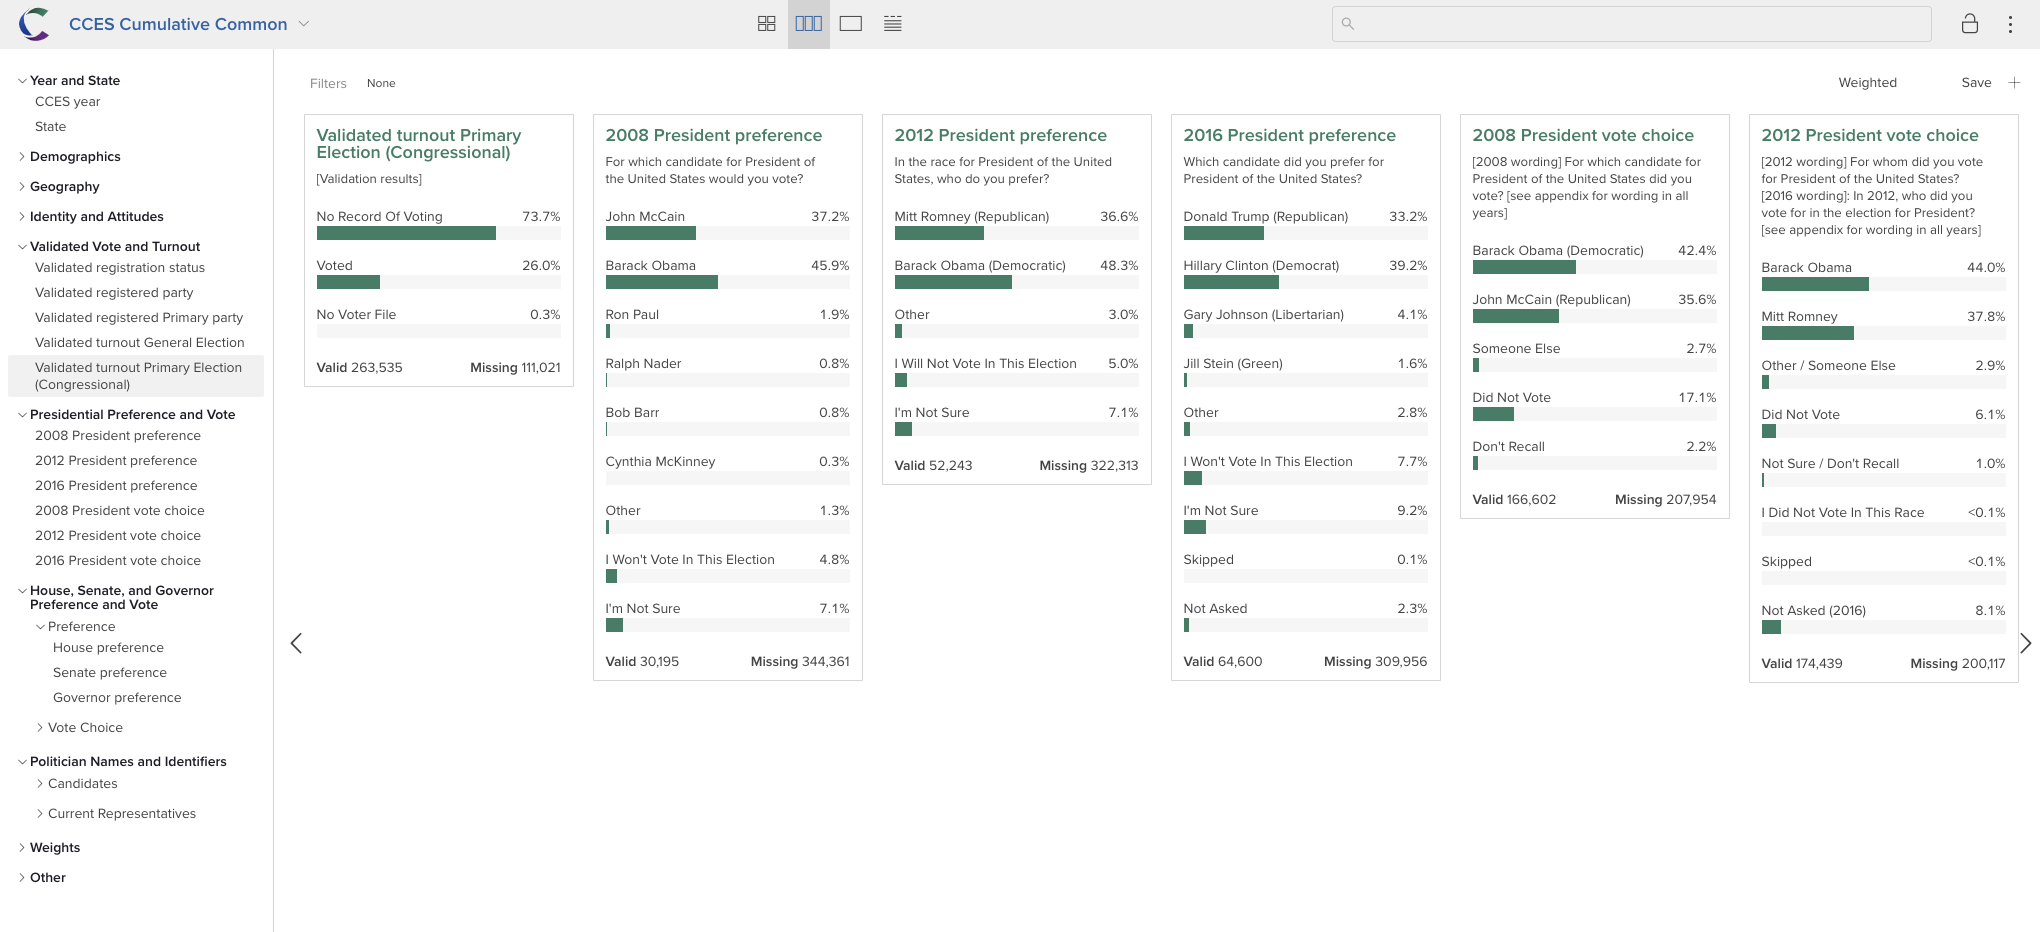
\includegraphics[width=1.05\linewidth]{01_crunch_browse.png}}
\end{figure}

\begin{enumerate}
\def\labelenumi{\arabic{enumi}.}
\setcounter{enumi}{2}
\tightlist
\item
  Analyze: The crunch interface allows Viewers to make cross-tabs and
  bar graphs quickly.\\

  \begin{figure}[H]
  \centering
  \centerline{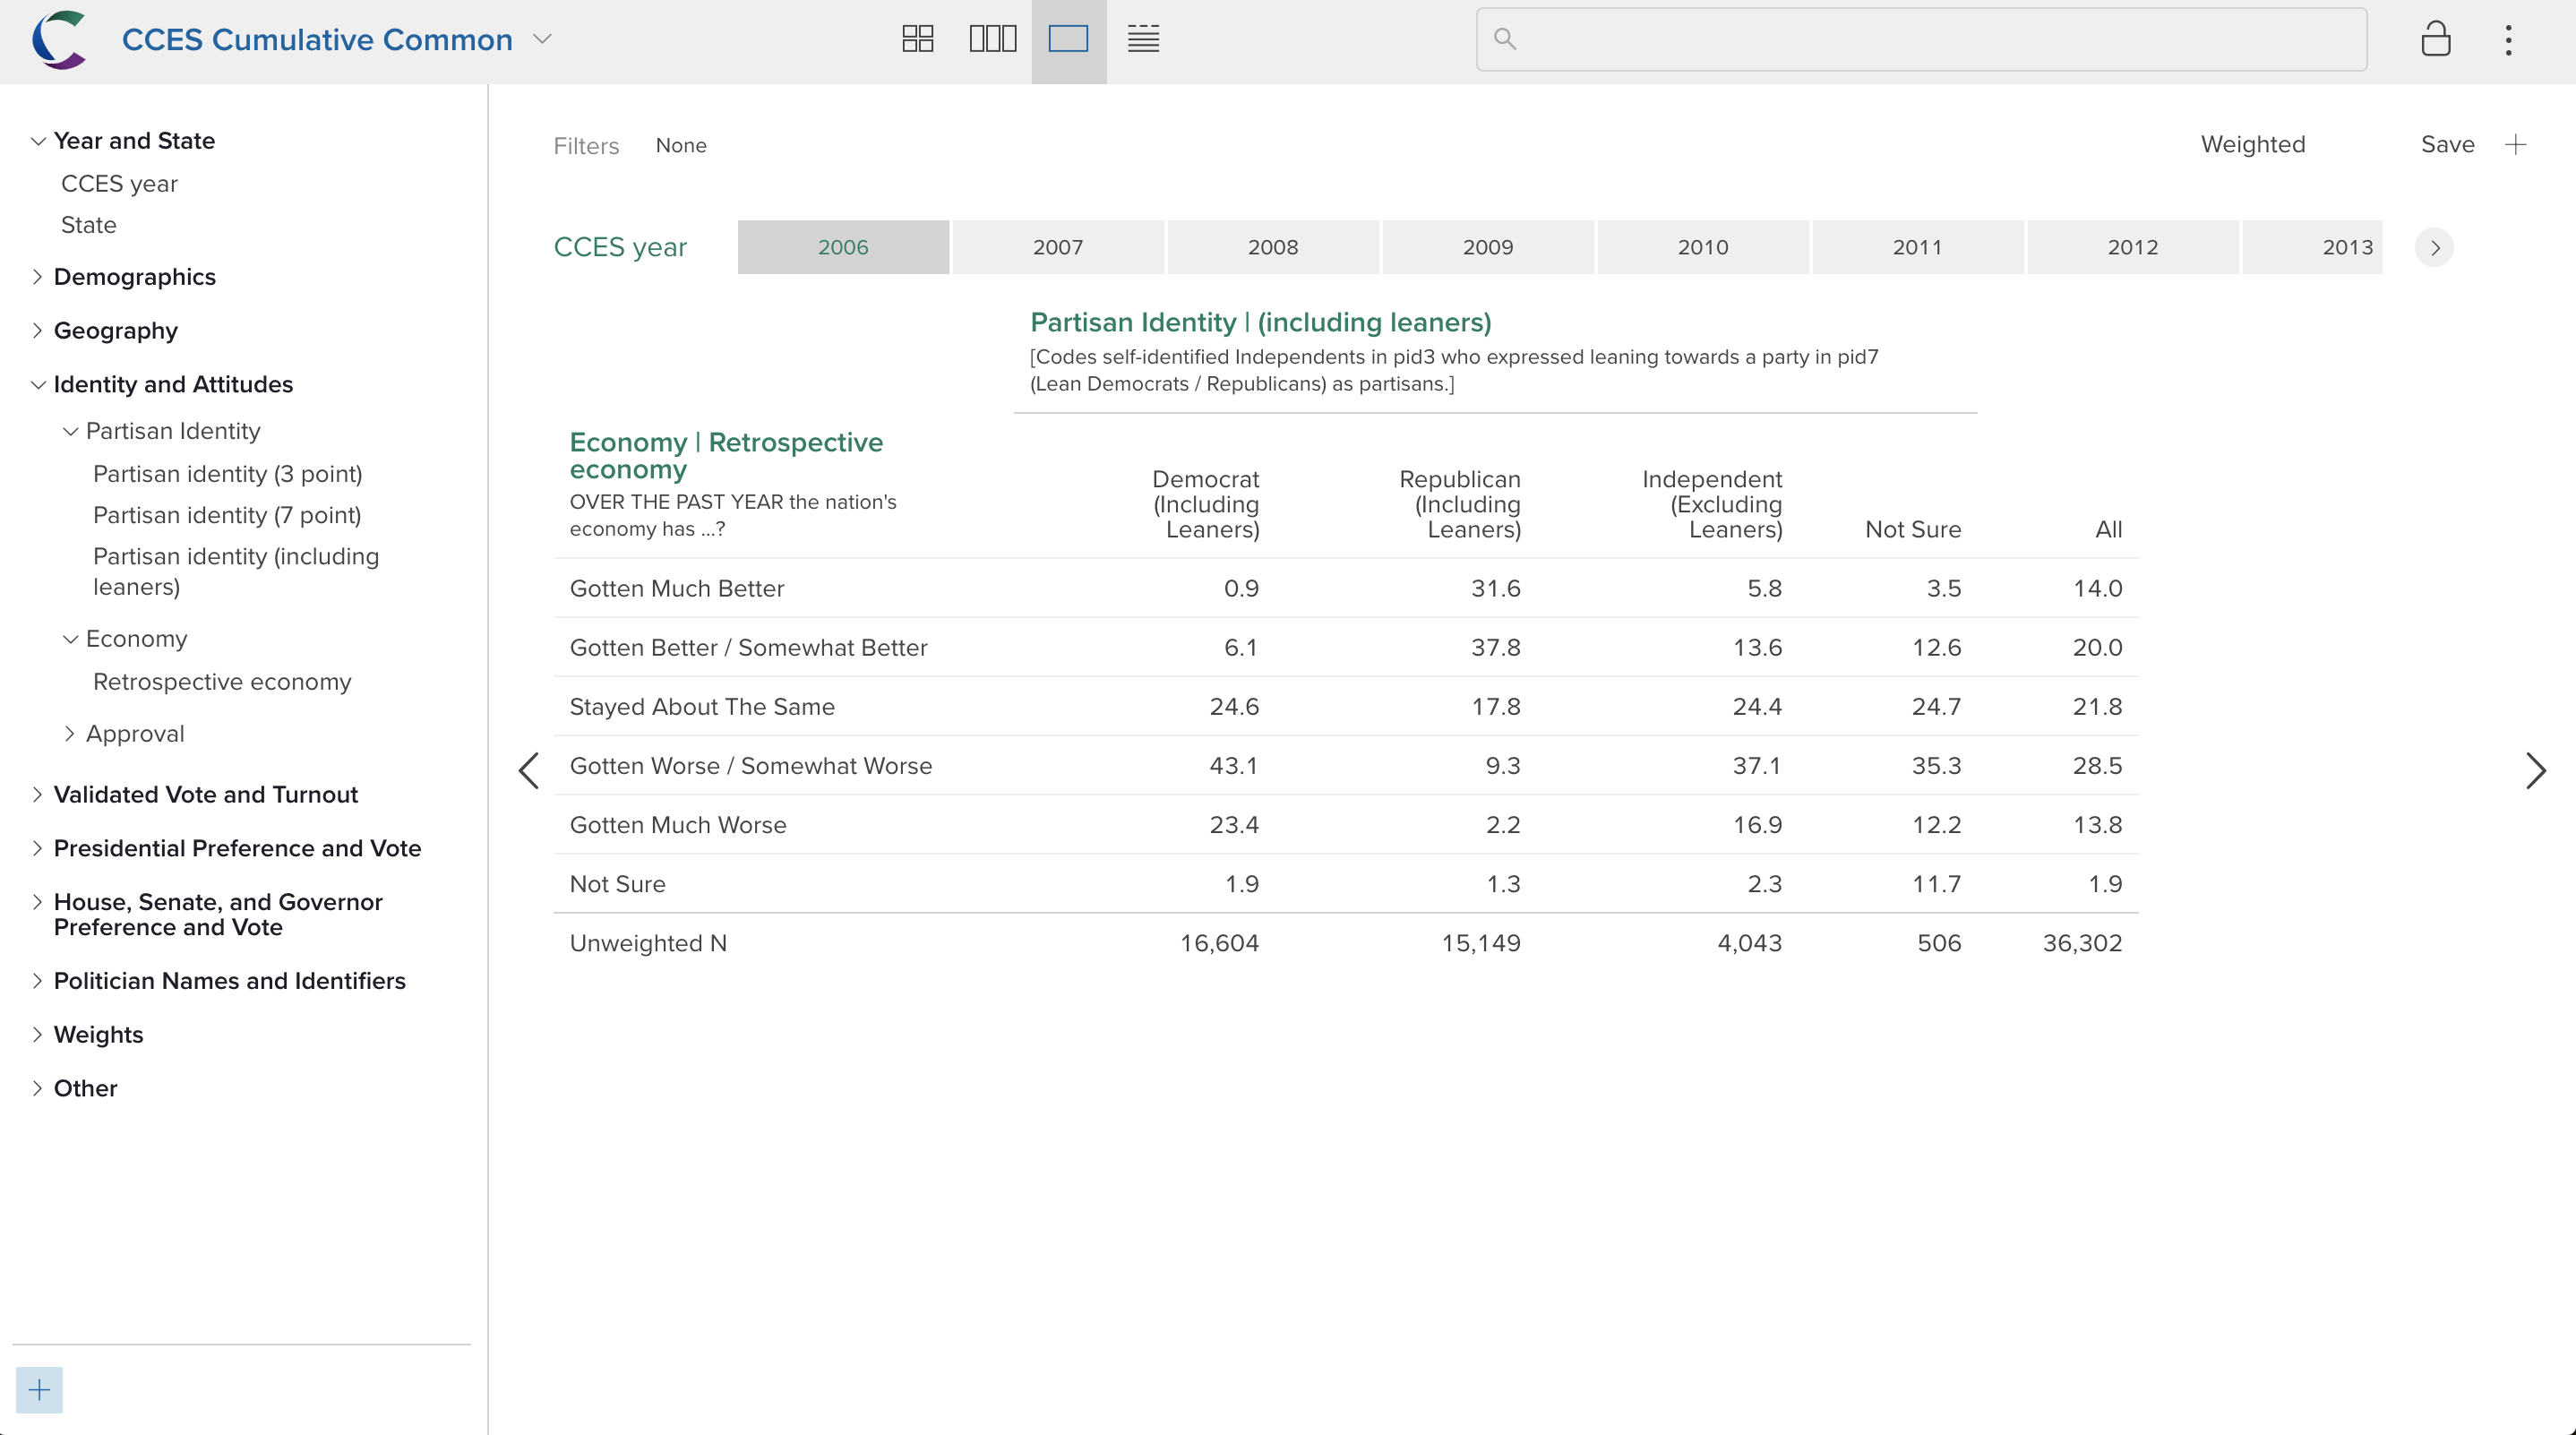
\includegraphics[width=1.05\linewidth]{02_crunch_tab.png}}
  \end{figure}
\end{enumerate}

Crunch datasets can also be manipulated from a R package,
\texttt{crunch}. To learn more about the features, please take a look at
their homepage \href{https://crunch.io}{crunch.io} or their
\href{https://www.youtube.com/watch?v=zA7N_Q1EpSs}{5-minute demo video}.

\newpage

\hypertarget{variables}{%
\section{Variables}\label{variables}}

The sections below provide summary statistics and more information on
each variable.

\begin{itemize}
\tightlist
\item
  The title shows the name of the variable as it appears in the dataset
  (``alias'' in Crunch terminology), followed by a more descriptive name
  suitable for presentation (``name'' in Crunch terminology).
\item
  Question wordings, where applicable, immediately follow. Otherwise a
  description is provided in square brackets (\texttt{{[}\ \ {]}}). All
  square brackets, both in the description and the response options,
  indicate descriptions that are summaries rather than the question
  verbatim.
\item
  A tabulation of response options (or summary statistics for numeric
  variables) follows. Numbers are unweighted counts.
\item
  The ``Years'' bullet lists the years of the CCES in which data on the
  variable is available at all. If a year is not listed, either the
  question was not asked in the year or was not incorporated in the
  creation of this dataset.
\item
  Finally, the ``Limitations'' bullet notes some of the caveats required
  when interpreting this variable. As this dataset is a combination of
  different surveys, some year-specific details on implementation are
  inevitably lost. For example, for all 2016 responses ``Not Asked'' and
  ``Skipped'' are both coded as a \texttt{NA} (missing) to stay
  consistent with past years that did not make that finer distinction.
\end{itemize}

\hypertarget{administration}{%
\subsection{Administration}\label{administration}}

\hypertarget{year-cces-year}{%
\subsubsection{\texorpdfstring{\texttt{year}: CCES
year}{year: CCES year}}\label{year-cces-year}}

{[}Year of CCES Common Content{]}

\begin{table}[H]
\centering
\begin{tabular}[t]{lr}
\toprule
 & n\\
\midrule
2006 & 36,421\\
2007 & 9,999\\
2008 & 32,800\\
2009 & 13,800\\
2010 & 55,400\\
2011 & 20,150\\
2012 & 54,535\\
2013 & 16,400\\
2014 & 56,200\\
2015 & 14,250\\
2016 & 64,600\\
2017 & 18,200\\
2018 & 60,000\\
2019 & 18,000\\
2020 & 61,000\\
2021 & 25,700\\
\bottomrule
\end{tabular}
\end{table}

\hypertarget{starttime-start-time}{%
\subsubsection{\texorpdfstring{\texttt{starttime}: Start
time}{starttime: Start time}}\label{starttime-start-time}}

{[}Pre-election wave start time (up to second){]}

\begin{table}
\centering
\begin{tabular}{lrr}
\toprule
 & Earliest Date & Latest Date\\
\midrule
2006 & 2006-10-07 & 2006-11-08\\
2007 & 2007-11-09 & 2007-12-10\\
2008 & 2008-10-08 & 2008-11-03\\
2009 & 2009-11-05 & 2009-12-14\\
2010 & 2010-10-01 & 2010-11-01\\
2011 & 2011-11-09 & 2012-01-07\\
2012 & 2012-10-01 & 2012-11-05\\
2013 & 2013-11-06 & 2013-12-03\\
2014 & 2014-10-01 & 2014-11-03\\
2015 & 2015-11-06 & 2015-12-03\\
2016 & 2016-09-28 & 2016-11-07\\
2017 & 2017-11-08 & 2017-12-12\\
2018 & 2018-09-27 & 2018-11-05\\
2019 & 2019-11-06 & 2019-12-05\\
2020 & 2020-09-29 & 2020-11-02\\
2021 & 2021-11-03 & 2021-12-07\\
\bottomrule
\end{tabular}
\end{table}

\begin{itemize}
\tightlist
\item
  Years: All of 2006-2021
\end{itemize}

\hypertarget{tookpost-took-post-election-wave}{%
\subsubsection{\texorpdfstring{\texttt{tookpost}: Took post-election
wave}{tookpost: Took post-election wave}}\label{tookpost-took-post-election-wave}}

{[}Whether or not the respondent took the post-election wave of the
survey (in even years){]}

\begin{table}[H]
\centering
\begin{tabular}[t]{lr}
\toprule
 & n\\
\midrule
Did Not Take Post-Election Survey & 68,513\\
Took Post-Election Survey & 352,443\\
(Missing) & 136,499\\
\bottomrule
\end{tabular}
\end{table}

\begin{itemize}
\tightlist
\item
  Years: 2006, 2008, 2010, 2012, 2014, 2016, 2018, 2020 (Post-election
  wave only exists for even years)
\end{itemize}

\hypertarget{weights}{%
\subsection{Weights}\label{weights}}

\hypertarget{weight-survey-weight-year-specific}{%
\subsubsection{\texorpdfstring{\texttt{weight}: Survey weight
(Year-Specific)}{weight: Survey weight (Year-Specific)}}\label{weight-survey-weight-year-specific}}

{[}weights for pre-election survey of each year{]}

\begin{verbatim}
   Min. 1st Qu.  Median    Mean 3rd Qu.    Max. 
 0.0000  0.4521  0.7349  1.0000  1.1624 15.0006 
\end{verbatim}

\begin{itemize}
\tightlist
\item
  Years: All of 2006-2021
\item
  In even years, they are re-computed after vote validation has been
  computed and those re-computed weights are taken here when available.
  The weights applied to the sample (which is originally drawn from a
  matched sample) are constructed to \textbf{make each year's data
  representative of the national adult population}. See the methodology
  section of the
  \href{https://dataverse.harvard.edu/api/access/datafile/3047286}{2016
  Guide} and the
  \href{https://cces.gov.harvard.edu/frequently-asked-questions}{FAQ on
  the CCES website} for details.
\item
  Limitations: Only specific to each year. Built off of the entire
  pre-election wave sample, but not necessarily to adjust post-election
  wave respondents. See \texttt{weight\_post}
\end{itemize}

\hypertarget{weight_cumulative-survey-weight-cumulative}{%
\subsubsection{\texorpdfstring{\texttt{weight\_cumulative}: Survey
weight
(Cumulative)}{weight\_cumulative: Survey weight (Cumulative)}}\label{weight_cumulative-survey-weight-cumulative}}

{[}weight variable with simple adjustment: multiplied a constant within
year to make years comparable{]}

\begin{verbatim}
   Min. 1st Qu.  Median    Mean 3rd Qu.    Max. 
 0.0000  0.2781  0.5000  0.8395  0.9720 21.4290 
\end{verbatim}

\begin{itemize}
\tightlist
\item
  Years: All of 2006-2021
\item
  Limitations: Only a simple transformation of \texttt{weight}.
  Specifically, \texttt{weight\_cumulative} is \texttt{weight} divided
  by the year-specific factors shown in the following table. For
  example, all weights in the 2016 common content are divided by about
  2.21, because it has about twice as many observations as the other
  datasets.
\item
  This transformation means that this simple cumulative weight makes
  sense when all years should be re-weighted to have the same sample
  size, even if that means doubling the weights. For analyses that are
  done year by year, using \texttt{weight} and
  \texttt{weight\_cumulative} are equivalent.
\end{itemize}

\begin{center}


\begin{tabular}{rrr}
\toprule
Year & Observations & Factor\\
\midrule
2006 & 36,421 & 1.25\\
2007 & 9,999 & 0.34\\
2008 & 32,800 & 1.12\\
2009 & 13,800 & 0.47\\
2010 & 55,400 & 1.89\\
2011 & 20,150 & 0.69\\
2012 & 54,535 & 1.86\\
2013 & 16,400 & 0.56\\
2014 & 56,200 & 1.92\\
2015 & 14,250 & 0.49\\
2016 & 64,600 & 2.21\\
2017 & 18,200 & 0.62\\
2018 & 60,000 & 2.05\\
2019 & 18,000 & 0.62\\
2020 & 61,000 & 2.09\\
2021 & 25,700 & 0.88\\
\bottomrule
\end{tabular}
\end{center}

\hypertarget{weight_post-survey-weight-for-post-election-wave}{%
\subsubsection{\texorpdfstring{\texttt{weight\_post}: Survey weight for
post-election
wave}{weight\_post: Survey weight for post-election wave}}\label{weight_post-survey-weight-for-post-election-wave}}

{[}weight for post-election wave respondents. Only available for some of
the even years.{]}

\begin{verbatim}
   Min. 1st Qu.  Median    Mean 3rd Qu.    Max.    NA's 
    0.0     0.5     0.7     1.0     1.1    15.0  356320 
\end{verbatim}

\begin{itemize}
\tightlist
\item
  Years: 2012, 2016, 2018, 2020
\item
  Limitations: Only available for some even years.
\item
  To analyze the post-election wave responses for years that do not have
  a post-specific weight, the second-best option is to use the normal
  \texttt{weight} variable. These weights will not be designed for the
  post-wave subset but they tend to correlate. When applying the weights
  to a subset of the data, make sure that they are rescaled to mean 1 in
  the non-missing subset (most statistical software will do this
  automatically).
\item
  To use the \texttt{weight\_post} for years it is available but
  \texttt{weight} for where it is not, one could coalesce into a new
  variable.
\end{itemize}

\hypertarget{rvweight-survey-weights-to-validated-registered-voters}{%
\subsubsection{\texorpdfstring{\texttt{rvweight}: Survey weights to
validated registered
voters}{rvweight: Survey weights to validated registered voters}}\label{rvweight-survey-weights-to-validated-registered-voters}}

{[}weights to validated registered voter population{]}

\begin{verbatim}
   Min. 1st Qu.  Median    Mean 3rd Qu.    Max.    NA's 
    0.0     0.6     0.8     1.0     1.2    16.3  474371 
\end{verbatim}

\begin{itemize}
\tightlist
\item
  Years: 2018, 2020
\item
  In 2018, YouGov computed weights after vote validation to weight to
  the target population of registered voters. See the methodology
  section of the \href{https://doi.org/10.7910/DVN/ZSBZ7K}{2018 Guide}
  for details. For this reason, and to distinguish it from the previous
  year's post-validation weights, the cumulative renames the 2018
  \texttt{vvweight} into \texttt{rvweight}.
\item
  Limitations: Only specific to each year. Built off of the entire
  pre-election wave sample, but not necessarily to adjust post-election
  wave respondents. See \texttt{rvweight\_post}
\end{itemize}

\hypertarget{rvweight_post-survey-weights-to-validated-registered-voters-post-election-wave}{%
\subsubsection{\texorpdfstring{\texttt{rvweight\_post}: Survey weights
to validated registered voters, post-election
wave}{rvweight\_post: Survey weights to validated registered voters, post-election wave}}\label{rvweight_post-survey-weights-to-validated-registered-voters-post-election-wave}}

{[}weights to validated registered voter population, post-election
wave{]}

\begin{verbatim}
   Min. 1st Qu.  Median    Mean 3rd Qu.    Max.    NA's 
    0.0     0.5     0.8     1.0     1.2    15.0  481492 
\end{verbatim}

\begin{itemize}
\tightlist
\item
  Years: 2018, 2020
\item
  Limitations: Only available for some even years.
\end{itemize}

\hypertarget{geography}{%
\subsection{Geography}\label{geography}}

A series of variables for the respondent's location:

\begin{itemize}
\tightlist
\item
  \texttt{state}: State (FIPS): {[}State{]}
\item
  \texttt{state\_post}: State (FIPS), post-election: {[}State,
  post-election{]}
\item
  \texttt{st}: State abbreviation (FIPS): {[}State Abbreviation{]}
\item
  \texttt{st\_post}: State abbreviation (FIPS), post-election: {[}State,
  post-election{]}
\item
  \texttt{dist}: Congressional district number in current Congress:
  {[}Current Congressional District Number{]}
\item
  \texttt{dist\_post}: Congressional district number in current
  Congress, post-election: {[}Current Congressional District Number,
  post-election{]}
\item
  \texttt{dist\_up}: Congressional district number for upcoming
  Congress: {[}Upcoming Congressional District Number{]}
\item
  \texttt{dist\_up\_post}: Congressional district number for upcoming
  Congress, post-election: {[}Upcoming Congressional District Number,
  post-election{]}
\item
  \texttt{cd}: Congressional district in current Congress: {[}Current
  Congressional District{]}
\item
  \texttt{cd\_post}: Congressional district in current Congress,
  post-election: {[}Current Congressional District, post-election{]}
\item
  \texttt{cd\_up}: Congressional district in upcoming Congress:
  {[}Upcoming Congressional District{]}
\item
  \texttt{cd\_up\_post}: Congressional district in upcoming Congress,
  post-election: {[}Upcoming Congressional District, post-election{]}
\item
  \texttt{zipcode}: Zipcode (lookupzip): {[}lookupzip in most years.{]}
  So that we can ask you about the news and events in your area, in what
  zip code do you currently reside?
\item
  \texttt{county\_fips}: County of residence: {[}County (Imputed from
  input zipcode){]}
\end{itemize}

\begin{verbatim}
Rows: 557,455
Columns: 14
$ state        <chr> "California", "Pennsylvania", "Texas", "Texas", "Texas", ~
$ st           <chr> "CA", "PA", "TX", "TX", "TX", "NY", "NC", "NC", "MA", "CA~
$ state_post   <chr> NA, "Pennsylvania", NA, "Texas", "Texas", "New York", NA,~
$ st_post      <chr> NA, "PA", NA, "TX", "TX", "NY", NA, NA, "MA", NA, "MI", "~
$ dist         <int> 2, 5, 16, 19, 6, 28, 11, 7, 1, 17, 15, 1, 2, 6, 1, 1, 16,~
$ dist_up      <int> 1, 3, 16, 19, 6, 27, 11, 7, 2, 20, 12, 1, 2, 8, 1, 1, 15,~
$ cd           <chr> "CA-02", "PA-05", "TX-16", "TX-19", "TX-06", "NY-28", "NC~
$ cd_up        <chr> "CA-01", "PA-03", "TX-16", "TX-19", "TX-06", "NY-27", "NC~
$ dist_post    <int> NA, 5, NA, 19, 6, 28, NA, NA, 1, NA, 15, 1, 2, NA, NA, NA~
$ dist_up_post <int> NA, 3, NA, 19, 6, 27, NA, NA, 2, NA, 12, 1, 2, NA, NA, NA~
$ cd_post      <chr> NA, "PA-05", NA, "TX-19", "TX-06", "NY-28", NA, NA, "MA-0~
$ cd_up_post   <chr> NA, "PA-03", NA, "TX-19", "TX-06", "NY-27", NA, NA, "MA-0~
$ zipcode      <chr> "95969", "16255", "79924", "79423", "76123", "14131", "28~
$ county_fips  <chr> "06007", "42031", "48141", "48303", "48439", "36063", "37~
\end{verbatim}

\begin{itemize}
\tightlist
\item
  Years: All of 2006-2021
\item
  Note the distinction between \texttt{dist} and \texttt{dist\_up},
  especially in 2012. The former should generally be used for linking
  respondents to their representatives at the time of the survey,
  whereas the latter can be used for the district in which they will
  vote for. New districts were drawn in 2010-2012 and candidates ran in
  new district maps in the 2012 CCES. Because respondents would not be
  \emph{represented} in the new district lines until January 2013, in
  the 2012 CCES \texttt{dist} is the old district line and
  \texttt{dist\_up} is the new district line for the General Election.
\item
  \texttt{zipcode} mostly relies on the variable often called
  \texttt{lookupzip} in each year's CCES. This is the zipcode of voter
  registration, or if not available, the residential zipcode, of the
  respondent. It is called lookup because it is used to look up the
  congressional district and other geographies of the respondent. For
  more information on zipcodes, see the CCES question.
\item
  Limitations: Some years do not provide the variable relevant to
  \texttt{dist\_up}, in which case the current district (\texttt{dist})
  is assigned automatically. Thus, \texttt{dist\_up} may not reflect
  district changes in off-cycle redistricting. Only residence (not
  registration) geographies included here; see individual years' for
  registration geographies.
\end{itemize}

\newpage

\hypertarget{demographics}{%
\subsection{Demographics}\label{demographics}}

\hypertarget{gender-gender}{%
\subsubsection{\texorpdfstring{\texttt{gender}:
Gender}{gender: Gender}}\label{gender-gender}}

``Are you male or female?''

\begin{table}[H]
\centering
\begin{tabular}[t]{lr}
\toprule
 & n\\
\midrule
Male & 243,740\\
Female & 288,015\\
(Missing) & 25,700\\
\bottomrule
\end{tabular}
\end{table}

\begin{itemize}
\tightlist
\item
  Years: All of 2006-2020
\end{itemize}

\hypertarget{birthyr-year-of-birth}{%
\subsubsection{\texorpdfstring{\texttt{birthyr}: Year of
birth}{birthyr: Year of birth}}\label{birthyr-year-of-birth}}

``In what year were you born?''

\begin{verbatim}
   Min. 1st Qu.  Median    Mean 3rd Qu.    Max. 
   1900    1951    1962    1965    1979    2003 
\end{verbatim}

\begin{itemize}
\tightlist
\item
  Years: All of 2006-2021
\end{itemize}

\hypertarget{age-age}{%
\subsubsection{\texorpdfstring{\texttt{age}:
Age}{age: Age}}\label{age-age}}

{[}Approximate age computed from the year of survey minus Year of
Birth{]}

\begin{verbatim}
   Min. 1st Qu.  Median    Mean 3rd Qu.    Max. 
  18.00   35.00   51.00   49.48   62.00  109.00 
\end{verbatim}

\begin{itemize}
\tightlist
\item
  Years: All of 2006-2021
\end{itemize}

\hypertarget{educ-education}{%
\subsubsection{\texorpdfstring{\texttt{educ}:
Education}{educ: Education}}\label{educ-education}}

``What is the highest level of education you have completed?''

\begin{table}[H]
\centering
\begin{tabular}[t]{lr}
\toprule
 & n\\
\midrule
No HS & 17,788\\
High School Graduate & 153,508\\
Some College & 135,513\\
2-Year & 55,386\\
4-Year & 126,748\\
Post-Grad & 68,445\\
(Missing) & 67\\
\bottomrule
\end{tabular}
\end{table}

\begin{itemize}
\tightlist
\item
  Years: All of 2006-2021
\end{itemize}

\hypertarget{race-race}{%
\subsubsection{\texorpdfstring{\texttt{race}:
Race}{race: Race}}\label{race-race}}

``What racial or ethnic group best describes you?''

\begin{table}[H]
\centering
\begin{tabular}[t]{lr}
\toprule
 & n\\
\midrule
White & 411,517\\
Black & 61,300\\
Hispanic & 46,416\\
Asian & 12,195\\
Native American & 4,476\\
Mixed & 11,395\\
Other & 9,291\\
Middle Eastern & 865\\
\bottomrule
\end{tabular}
\end{table}

\begin{itemize}
\tightlist
\item
  Years: All of 2006-2021
\item
  Limitations: The ``Hispanic'' value may undercount self-identified
  Hispanics. See \texttt{hispanic}
\end{itemize}

\hypertarget{hispanic-hispanic}{%
\subsubsection{\texorpdfstring{\texttt{hispanic}:
Hispanic}{hispanic: Hispanic}}\label{hispanic-hispanic}}

``Are you of Spanish, Latino, or Hispanic origin or descent? {[}Asked if
response to race is not Hispanic{]}''

\begin{table}[H]
\centering
\begin{tabular}[t]{lr}
\toprule
 & n\\
\midrule
Yes & 14,183\\
No & 412,978\\
(Missing) & 130,294\\
\bottomrule
\end{tabular}
\end{table}

\begin{itemize}
\tightlist
\item
  Years: 2010, 2011, 2012, 2013, 2014, 2015, 2016, 2017, 2018, 2019,
  2020, 2021
\item
  In years in which this question was fielded, this question supplements
  the \texttt{race} variable by asking those who did \emph{not} respond
  ``Hipsanic'' in the \texttt{race} question.
\end{itemize}

\hypertarget{citizen-citizenship}{%
\subsubsection{\texorpdfstring{\texttt{citizen}:
Citizenship}{citizen: Citizenship}}\label{citizen-citizenship}}

{[}Based on self-report for immigration status{]}

\begin{table}[H]
\centering
\begin{tabular}[t]{lr}
\toprule
 & n\\
\midrule
Citizen & 522,904\\
Non-Citizen & 8,554\\
(Missing) & 25,997\\
\bottomrule
\end{tabular}
\end{table}

\begin{itemize}
\tightlist
\item
  Years: 2006, 2008, 2009, 2010, 2011, 2012, 2013, 2014, 2016, 2017,
  2018, 2019, 2020, 2021
\item
  These come from the immigration status questions, which ask
  respondents between first, second, and third generation citizens, and
  other foreign-born citizens. Here we mark anyone who does not answer
  the last category to be a citizen.
\item
  Limitation: Most of the missingness comes from 2007 and 2015, when the
  immigration status question does not appear to have been asked.
\end{itemize}

\hypertarget{religion-religion}{%
\subsubsection{\texorpdfstring{\texttt{religion}:
Religion}{religion: Religion}}\label{religion-religion}}

``What is your present religion, if any?''

\begin{table}[H]
\centering
\begin{tabular}[t]{lr}
\toprule
 & n\\
\midrule
Protestant & 196,298\\
Roman Catholic & 106,832\\
Mormon & 7,745\\
Eastern or Greek Orthodox & 2,686\\
Jewish & 12,977\\
Muslim & 2,678\\
Buddhist & 4,414\\
Hindu & 1,496\\
Atheist & 26,839\\
Agnostic & 30,112\\
Nothing in Particular & 93,508\\
Something Else & 34,412\\
(Missing) & 37,458\\
\bottomrule
\end{tabular}
\end{table}

\begin{itemize}
\tightlist
\item
  Years: 2007, 2008, 2009, 2010, 2011, 2012, 2013, 2014, 2015, 2016,
  2017, 2018, 2019, 2020, 2021
\item
  The response options have stayed largely consistent and follow that of
  Pew.
\end{itemize}

\hypertarget{family-status}{%
\subsection{Family Status}\label{family-status}}

\hypertarget{marstat-marital-status}{%
\subsubsection{\texorpdfstring{\texttt{marstat}: Marital
Status}{marstat: Marital Status}}\label{marstat-marital-status}}

``What is your marital status?''

\begin{table}[H]
\centering
\begin{tabular}[t]{lr}
\toprule
 & n\\
\midrule
Married & 299,885\\
Separated & 9,421\\
Divorced & 61,242\\
Widowed & 26,855\\
Single / Never Married & 131,650\\
Domestic Partnership & 26,816\\
(Missing) & 1,586\\
\bottomrule
\end{tabular}
\end{table}

\begin{itemize}
\tightlist
\item
  Years: All of 2006-2021
\item
  The option ``Single'' was used till 2016, which was then replaced by
  ``Never Married'' in 2017 and 2018.
\item
  The option ``Domestic Partnership'' was used till 2016, which was then
  replaced by ``Domestic / Civil Partnership'' in 2017 and 2018.
\end{itemize}

\hypertarget{ownhome-home-ownership}{%
\subsubsection{\texorpdfstring{\texttt{ownhome}: Home
Ownership}{ownhome: Home Ownership}}\label{ownhome-home-ownership}}

``Do you own your home or pay rent?''

\begin{table}[H]
\centering
\begin{tabular}[t]{lr}
\toprule
 & n\\
\midrule
Own & 331,034\\
Rent & 158,907\\
Other & 22,442\\
(Missing) & 45,072\\
\bottomrule
\end{tabular}
\end{table}

\begin{itemize}
\tightlist
\item
  Years: 2006, 2009, 2010, 2011, 2012, 2013, 2014, 2015, 2016, 2017,
  2018, 2019, 2020, 2021
\end{itemize}

\hypertarget{has_child-parent-of-young-children}{%
\subsubsection{\texorpdfstring{\texttt{has\_child}: Parent of Young
Children}{has\_child: Parent of Young Children}}\label{has_child-parent-of-young-children}}

``Are you the parent or guardian of any children under the age of 18?''

\begin{table}[H]
\centering
\begin{tabular}[t]{lr}
\toprule
 & n\\
\midrule
Yes & 128,036\\
No & 382,035\\
(Missing) & 47,384\\
\bottomrule
\end{tabular}
\end{table}

\begin{itemize}
\tightlist
\item
  Years: 2008, 2009, 2010, 2011, 2012, 2013, 2014, 2015, 2016, 2017,
  2018, 2019, 2020, 2021
\end{itemize}

\hypertarget{no_milstat-military-status-none}{%
\subsubsection{\texorpdfstring{\texttt{no\_milstat}: Military Status
(None)}{no\_milstat: Military Status (None)}}\label{no_milstat-military-status-none}}

{[}Based on military household question; neither respondent nor
immediate family has served{]}

\begin{table}[H]
\centering
\begin{tabular}[t]{lr}
\toprule
 & n\\
\midrule
Yes & 231,870\\
No & 315,491\\
(Missing) & 10,094\\
\bottomrule
\end{tabular}
\end{table}

\begin{itemize}
\tightlist
\item
  Years: 2006, 2008, 2009, 2010, 2011, 2012, 2013, 2014, 2015, 2016,
  2017, 2018, 2019, 2020, 2021
\item
  The original question is of the form ``We'd like to know whether you
  or someone in your immediate family is currently serving or has ever
  served in the U.S. military. Immediate family is defined as your
  parents, siblings, spouse, and children. Please check all boxes that
  apply.'', where respondents can pick more than one of the options
  including the following: ``I served personally'', ``Family served
  previously''. The entry in the cumulative response only selects the
  ``None'' option. A value of \texttt{no\_milstat\ ==\ "Yes"} means that
  a respondent indicated they had neither served nor had an immediate
  family member who has served. To see the other responses, see the
  individual year's CCES.
\end{itemize}

\newpage

\hypertarget{validations}{%
\subsection{Validations}\label{validations}}

Observations in even years include indicators for validated voting,
which means that YouGov has matched survey respondents' personal
identifiable information to public voter files, which in turn officially
record whether a person has voted or not. Validation is often completed
in the summer following the election. For more information, see
\href{https://doi.org/10.1093/pan/mps023}{Ansolabehere and Hersh
(2012)}.

\hypertarget{vv_regstatus-validated-registration-status}{%
\subsubsection{\texorpdfstring{\texttt{vv\_regstatus}: Validated
registration
status}{vv\_regstatus: Validated registration status}}\label{vv_regstatus-validated-registration-status}}

{[}Validation results. Missing if validation was not conducted in the
year. Categories are aggregated. Both Matched-not registered and
unmatched are labeled as a no record.{]}

\begin{table}[H]
\centering
\begin{tabular}[t]{lr}
\toprule
 & n\\
\midrule
Active & 261,440\\
No Record of Registration & 90,341\\
Unregistered & 18,070\\
Dropped & 8,433\\
Inactive & 4,086\\
Multiple Appearances & 2,165\\
(Missing) & 172,920\\
\bottomrule
\end{tabular}
\end{table}

\begin{itemize}
\tightlist
\item
  Years: 2008, 2010, 2012, 2014, 2016, 2018, 2020
\item
  Limitations: Collapses some response options
\end{itemize}

\hypertarget{vv_party_gen-validated-registered-party}{%
\subsubsection{\texorpdfstring{\texttt{vv\_party\_gen}: Validated
registered
party}{vv\_party\_gen: Validated registered party}}\label{vv_party_gen-validated-registered-party}}

{[}Validation results. Only available for some states and years{]}

\begin{table}[H]
\centering
\begin{tabular}[t]{lr}
\toprule
 & n\\
\midrule
No Record of Party Registration & 94,627\\
Unknown & 87,810\\
Democratic Party & 50,181\\
Republican Party & 37,148\\
No Party Affiliation & 18,380\\
Declined to State & 3,093\\
Other & 2,015\\
Independent Party & 1,851\\
Libertarian Party & 726\\
Green Party & 341\\
Cns & 77\\
Constitution Party & 47\\
Wor & 19\\
Reform Party & 13\\
Socialist Party & 7\\
(Missing) & 261,120\\
\bottomrule
\end{tabular}
\end{table}

\begin{itemize}
\tightlist
\item
  Years: 2012, 2014, 2016, 2018, 2020
\item
  Limitations: Note that if the state's voter roll does not record party
  registration, this value will be missing. Not available for some even
  years.
\end{itemize}

\hypertarget{vv_party_prm-validated-registered-primary-party}{%
\subsubsection{\texorpdfstring{\texttt{vv\_party\_prm}: Validated
registered Primary
party}{vv\_party\_prm: Validated registered Primary party}}\label{vv_party_prm-validated-registered-primary-party}}

{[}Validation results. Only available for some states and years{]}

\begin{table}[H]
\centering
\begin{tabular}[t]{lr}
\toprule
 & n\\
\midrule
No Record of Party Registration & 256,215\\
Democratic Party & 21,325\\
Republican Party & 18,723\\
Libertarian Party & 29\\
No Party Affiliation & 27\\
Green Party & 6\\
Other & 9\\
Independent Party & 1\\
(Missing) & 261,120\\
\bottomrule
\end{tabular}
\end{table}

\begin{itemize}
\tightlist
\item
  Years: 2012, 2014, 2016, 2018, 2020
\item
  Limitations: Not available for some even years
\end{itemize}

\newpage

\hypertarget{turnout}{%
\subsection{Turnout}\label{turnout}}

\hypertarget{vv_turnout_gvm-validated-turnout-general-election}{%
\subsubsection{\texorpdfstring{\texttt{vv\_turnout\_gvm}: Validated
turnout General
Election}{vv\_turnout\_gvm: Validated turnout General Election}}\label{vv_turnout_gvm-validated-turnout-general-election}}

{[}Validation results. All vote methods (polling, mail, early, unknown,
etc..) are aggregated as a vote.{]}

\begin{table}[H]
\centering
\begin{tabular}[t]{lr}
\toprule
 & n\\
\midrule
Voted & 242,164\\
No Record of Voting & 177,059\\
No Voter File & 1,733\\
(Missing) & 136,499\\
\bottomrule
\end{tabular}
\end{table}

\begin{itemize}
\tightlist
\item
  Years: 2006, 2008, 2010, 2012, 2014, 2016, 2018, 2020
\item
  Limitations: Collapses most response options. For example, the
  particular voting method is collapsed into one category, even though
  \texttt{gvm} stands for General Election voting \emph{method}. Also,
  the result of not matching to a voter file is collapsed with the
  result of matching to a voter file and having no indication of turning
  out to vote. The distinction is unclear in earlier years, and is thus
  collapsed for all years here. For finer distinctions, see the
  individual year's CCES.
\end{itemize}

\hypertarget{vv_turnout_pvm-validated-turnout-primary-election-congressional}{%
\subsubsection{\texorpdfstring{\texttt{vv\_turnout\_pvm}: Validated
turnout Primary Election
(Congressional)}{vv\_turnout\_pvm: Validated turnout Primary Election (Congressional)}}\label{vv_turnout_pvm-validated-turnout-primary-election-congressional}}

{[}Validation results. Congressional primaries.{]}

\begin{table}[H]
\centering
\begin{tabular}[t]{lr}
\toprule
 & n\\
\midrule
No Record of Voting & 260,715\\
Voted & 122,457\\
No Voter File & 1,363\\
(Missing) & 172,920\\
\bottomrule
\end{tabular}
\end{table}

\begin{itemize}
\tightlist
\item
  Years: 2008, 2010, 2012, 2014, 2016, 2018, 2020
\item
  Limitations: See \texttt{vv\_turnout\_gvm}
\end{itemize}

\hypertarget{intent_turnout_self-self-reported-turnout-pre-election-wave}{%
\subsubsection{\texorpdfstring{\texttt{intent\_turnout\_self}:
Self-reported turnout (pre-election
wave)}{intent\_turnout\_self: Self-reported turnout (pre-election wave)}}\label{intent_turnout_self-self-reported-turnout-pre-election-wave}}

``2020: Do you intend to vote in the 2020 general election on November
3rd?''

\begin{table}[H]
\centering
\begin{tabular}[t]{lr}
\toprule
 & n\\
\midrule
Yes, definitely & 206,578\\
Probably & 22,893\\
I already voted (early or absentee) & 20,699\\
Plan to vote early & 6,541\\
No & 23,162\\
Undecided & 16,122\\
(Missing) & 261,460\\
\bottomrule
\end{tabular}
\end{table}

\begin{itemize}
\tightlist
\item
  Years: 2012, 2014, 2016, 2018, 2020
\item
  Limitations: Collapses and simplifies response categories to
  standardize across years. See individual year's datasets for details.
  Some response categories are still not standardized. For example,
  ``Plan to vote early'' was not an option only in 2016. Additionally,
  the question is available in years 2010 and earlier but not included
  in this version of the cumulative dataset because those years rely on
  a 2006--2012 cumulative release.
\end{itemize}

\hypertarget{voted_turnout_self-self-reported-turnout-post-election-wave}{%
\subsubsection{\texorpdfstring{\texttt{voted\_turnout\_self}:
Self-reported turnout (post-election
wave)}{voted\_turnout\_self: Self-reported turnout (post-election wave)}}\label{voted_turnout_self-self-reported-turnout-post-election-wave}}

``2020: Which of the following statements best describes you?''

\begin{table}[H]
\centering
\begin{tabular}[t]{lr}
\toprule
 & n\\
\midrule
Yes & 303,222\\
No & 40,591\\
(Missing) & 213,642\\
\bottomrule
\end{tabular}
\end{table}

\begin{itemize}
\tightlist
\item
  Years: 2006, 2008, 2010, 2012, 2014, 2016, 2018, 2020
\item
  Limitations: Collapses reasons for not voting into a single ``No''.
  Actual responses distinguish between ``Did not vote'' and ``Tried to
  vote but could not'' in some years, for example. To standardize across
  years, the cumulative dataset lumps these levels and others together.
  See the individual year's datasets for details. The cumulative dataset
  also does not include responses for odd years even though in some odd
  years this question is asked.
\end{itemize}

\newpage

\hypertarget{partisan-identity}{%
\subsection{Partisan Identity}\label{partisan-identity}}

\hypertarget{pid3-partisan-identity-3-point}{%
\subsubsection{\texorpdfstring{\texttt{pid3}: Partisan identity (3
point)}{pid3: Partisan identity (3 point)}}\label{pid3-partisan-identity-3-point}}

``Generally speaking, do you think of yourself as a \ldots?''

\begin{table}[H]
\centering
\begin{tabular}[t]{lr}
\toprule
 & n\\
\midrule
Democrat & 202,454\\
Republican & 146,432\\
Independent & 158,103\\
Other & 22,618\\
Not Sure & 27,607\\
(Missing) & 241\\
\bottomrule
\end{tabular}
\end{table}

\begin{itemize}
\tightlist
\item
  Years: All of 2006-2021
\item
  Limitations: Response options offer slightly by year. For example, the
  \texttt{Not\ Sure} option is not a response option in years 2006 and
  2010. Open-text responses not included. 2010 values are from the
  post-election wave. 2020 values do not include the \texttt{Not\ Sure}
  option (option 5).
\end{itemize}

\hypertarget{pid7-partisan-identity-7-point}{%
\subsubsection{\texorpdfstring{\texttt{pid7}: Partisan identity (7
point)}{pid7: Partisan identity (7 point)}}\label{pid7-partisan-identity-7-point}}

{[}Based on branching from Partisan Identity question{]}

\begin{table}[H]
\centering
\begin{tabular}[t]{lr}
\toprule
 & n\\
\midrule
Strong Democrat & 135,271\\
Not Very Strong Democrat & 66,539\\
Lean Democrat & 56,265\\
Independent & 76,826\\
Lean Republican & 56,565\\
Not Very Strong Republican & 52,410\\
Strong Republican & 93,383\\
Not Sure & 17,161\\
Don't Know & 3\\
(Missing) & 3,032\\
\bottomrule
\end{tabular}
\end{table}

\begin{itemize}
\tightlist
\item
  Years: All of 2006-2021
\item
  Limitations: See \texttt{pid3}
\end{itemize}

\hypertarget{pid3_leaner-partisan-identity-including-leaners}{%
\subsubsection{\texorpdfstring{\texttt{pid3\_leaner}: Partisan identity
(including
leaners)}{pid3\_leaner: Partisan identity (including leaners)}}\label{pid3_leaner-partisan-identity-including-leaners}}

{[}Codes self-identified Independents in pid3 who expressed leaning
towards a party in pid7 (Lean Democrats / Republicans) as partisans.{]}

\begin{table}[H]
\centering
\begin{tabular}[t]{lr}
\toprule
 & n\\
\midrule
Democrat (Including Leaners) & 258,075\\
Republican (Including Leaners) & 202,358\\
Independent (Excluding Leaners) & 76,826\\
Not Sure & 17,161\\
(Missing) & 3,035\\
\bottomrule
\end{tabular}
\end{table}

\begin{itemize}
\tightlist
\item
  Years: All of 2006-2021
\item
  Limitations: See \texttt{pid3}
\end{itemize}

\hypertarget{ideo5-ideology-5-point}{%
\subsubsection{\texorpdfstring{\texttt{ideo5}: Ideology (5
point)}{ideo5: Ideology (5 point)}}\label{ideo5-ideology-5-point}}

``In general, how would you describe your own political viewpoint?''

\begin{table}[H]
\centering
\begin{tabular}[t]{lr}
\toprule
 & n\\
\midrule
Very Liberal & 54,456\\
Liberal & 98,744\\
Moderate & 173,972\\
Conservative & 123,806\\
Very Conservative & 64,573\\
Not Sure & 40,065\\
(Missing) & 1,839\\
\bottomrule
\end{tabular}
\end{table}

\begin{itemize}
\tightlist
\item
  Years: All of 2006-2021
\end{itemize}

\hypertarget{economics-and-income}{%
\subsection{Economics and Income}\label{economics-and-income}}

\hypertarget{faminc-family-income}{%
\subsubsection{\texorpdfstring{\texttt{faminc}: Family
Income}{faminc: Family Income}}\label{faminc-family-income}}

``Thinking back over the last year, what was your family's annual
income? {[}Brackets coarsened{]}''

\begin{table}[H]
\centering
\begin{tabular}[t]{lr}
\toprule
 & n\\
\midrule
Less than 10k & 25,095\\
10k - 20k & 41,126\\
20k - 30k & 56,343\\
30k - 40k & 56,675\\
40k - 50k & 50,652\\
50k - 60k & 49,346\\
60k - 70k & 36,508\\
70k - 80k & 39,964\\
80k - 100k & 46,268\\
100k - 120k & 33,788\\
120k - 150k & 27,860\\
150k+ & 32,598\\
Prefer not to say & 59,639\\
Skipped & 12\\
(Missing) & 1,581\\
\bottomrule
\end{tabular}
\end{table}

\begin{itemize}
\tightlist
\item
  Years: All of 2006-2021
\item
  Limitations: The income brackets provided changed slightly over time.
  The brackets in this cumulative dataset coarsen certain original
  brackets, losing some granularity. In particular, from 2011-2016,
  respondents answering ``over 150k'' were asked a follow-up question to
  select one of several brackets above 150k. Here, these are top-coded
  and only labelled as ``over 150k.''
\item
  The 2009 CCES did not have an option for 60-70k.
\end{itemize}

\hypertarget{employ-employment-status}{%
\subsubsection{\texorpdfstring{\texttt{employ}: Employment
Status}{employ: Employment Status}}\label{employ-employment-status}}

``Which of the following best describes your current employment
status?''

\begin{table}[H]
\centering
\begin{tabular}[t]{lr}
\toprule
 & n\\
\midrule
Full-Time & 218,830\\
Part-Time & 57,248\\
Temporarily Laid Off & 4,827\\
Unemployed & 36,710\\
Retired & 118,985\\
Permanently Disabled & 33,141\\
Homemaker & 39,749\\
Student & 24,441\\
Other & 13,232\\
(Missing) & 10,292\\
\bottomrule
\end{tabular}
\end{table}

\begin{itemize}
\tightlist
\item
  Years: 2006, 2008, 2009, 2010, 2011, 2012, 2013, 2014, 2015, 2016,
  2017, 2018, 2019, 2020, 2021
\end{itemize}

\hypertarget{no_healthins-uninsured}{%
\subsubsection{\texorpdfstring{\texttt{no\_healthins}:
Uninsured}{no\_healthins: Uninsured}}\label{no_healthins-uninsured}}

{[}Based on health insurance question; respondent has none of the
insurance options given{]}

\begin{table}[H]
\centering
\begin{tabular}[t]{lr}
\toprule
 & n\\
\midrule
Yes & 52,330\\
No & 425,841\\
(Missing) & 79,284\\
\bottomrule
\end{tabular}
\end{table}

\begin{itemize}
\tightlist
\item
  Years: 2009, 2010, 2011, 2012, 2013, 2014, 2015, 2016, 2017, 2018,
  2019, 2020, 2021
\item
  The original question is of the form ``Do you currently have health
  insurance? (check all that apply)'', where respondents can pick more
  than one of the options including the following: ``Yes, through my job
  or a family member's employer'', ``Yes, through a government program,
  such as Medicare or Medicaid''. The entry in the cumulative response
  only selects the ``None'' option. A value of
  \texttt{no\_healthins\ ==\ "Yes"} means that a respondent indicated
  they were not insured. To see the other responses, see the individual
  year's CCES.
\end{itemize}

\hypertarget{union-union-membership}{%
\subsubsection{\texorpdfstring{\texttt{union}: Union
membership}{union: Union membership}}\label{union-union-membership}}

``Are you a member of a union?''

\begin{table}[H]
\centering
\begin{tabular}[t]{lr}
\toprule
 & n\\
\midrule
Yes, Currently & 35,912\\
Yes, Formerly & 104,008\\
No, Never & 373,488\\
(Missing) & 44,047\\
\bottomrule
\end{tabular}
\end{table}

\begin{itemize}
\tightlist
\item
  Years: 2006, 2009, 2010, 2011, 2012, 2013, 2014, 2015, 2016, 2017,
  2018, 2019, 2020, 2021
\item
  Question wording and response options have been reworded to be
  harmonized across years. Please see each individual CCES for exact
  wording.
\item
  The 2008 CCES in its common content has a union question that roughly
  combines both the \texttt{union} and \texttt{union\_hh} question.
\end{itemize}

\hypertarget{union_hh-union-membership-in-household}{%
\subsubsection{\texorpdfstring{\texttt{union\_hh}: Union membership in
household}{union\_hh: Union membership in household}}\label{union_hh-union-membership-in-household}}

``Other than yourself, is any member of your household a union member?''

\begin{table}[H]
\centering
\begin{tabular}[t]{lr}
\toprule
 & n\\
\midrule
Yes, Currently & 46,422\\
Yes, Formerly & 73,616\\
No, Never & 387,107\\
Not Sure & 3,576\\
(Missing) & 46,734\\
\bottomrule
\end{tabular}
\end{table}

\begin{itemize}
\tightlist
\item
  Years: 2006, 2009, 2010, 2011, 2012, 2013, 2014, 2015, 2016, 2017,
  2018, 2019, 2020, 2021
\item
  Question wording and response options have been reworded to be
  harmonized across years. Please see each individual CCES for exact
  wording.
\item
  The 2008 CCES in its common content has a union question that roughly
  combines both the \texttt{union} and \texttt{union\_hh} question.
\end{itemize}

\hypertarget{economy_retro-retrospective-economy}{%
\subsubsection{\texorpdfstring{\texttt{economy\_retro}: Retrospective
economy}{economy\_retro: Retrospective economy}}\label{economy_retro-retrospective-economy}}

``OVER THE PAST YEAR the nation's economy has \ldots?''

\begin{table}[H]
\centering
\begin{tabular}[t]{lr}
\toprule
 & n\\
\midrule
Gotten much better & 38,344\\
Gotten better / somewhat better & 116,370\\
Stayed about the same & 135,629\\
Gotten worse / somewhat worse & 139,478\\
Gotten much worse & 112,158\\
Not sure & 14,433\\
(Missing) & 1,043\\
\bottomrule
\end{tabular}
\end{table}

\begin{itemize}
\tightlist
\item
  Years: All of 2006-2021
\item
  Limitations: Response options vary by year. Some are collapsed into
  one category (e.g., \texttt{Gotten\ Better}, presented in some years,
  and \texttt{Gotten\ Somewhat\ Better}, presented in other years, are
  collapsed into \texttt{Gotten\ Better\ /\ Somewhat\ Better}). Some are
  left as is. For example, \texttt{Not\ Sure} was not an option in 2009.
\end{itemize}

\hypertarget{news-interest}{%
\subsection{News Interest}\label{news-interest}}

\hypertarget{newsint-news-interest}{%
\subsubsection{\texorpdfstring{\texttt{newsint}: News
Interest}{newsint: News Interest}}\label{newsint-news-interest}}

``Some people seem to follow what's going on in government and public
affairs most of the time, whether there's an election going on or not.
Others aren't that interested. Would you say you follow what's going on
in government and public affairs ..''

\begin{table}[H]
\centering
\begin{tabular}[t]{lr}
\toprule
 & n\\
\midrule
Most of the time & 279,220\\
Some of the time & 132,404\\
Only now and then & 62,826\\
Hardly at all & 31,998\\
Don't Know & 13,937\\
(Missing) & 37,070\\
\bottomrule
\end{tabular}
\end{table}

\begin{itemize}
\tightlist
\item
  Years: 2007, 2008, 2009, 2010, 2011, 2012, 2013, 2014, 2015, 2016,
  2017, 2018, 2019, 2020, 2021
\item
  Limitations: Not asked in 2006. Similar questions about watching TV
  news was asked in 2006, but not included in this cumulative file.
\end{itemize}

\hypertarget{approval}{%
\subsection{Approval}\label{approval}}

\hypertarget{approval_pres-president-approval}{%
\subsubsection{\texorpdfstring{\texttt{approval\_pres}: President
approval}{approval\_pres: President approval}}\label{approval_pres-president-approval}}

``Do you approve of the way each is doing their job\ldots{} {[}Pipe
Incumbent President{]}''

\begin{table}[H]
\centering
\begin{tabular}[t]{lr}
\toprule
 & n\\
\midrule
Strongly Approve & 117,770\\
Approve / Somewhat Approve & 123,054\\
Disapprove / Somewhat Disapprove & 55,313\\
Strongly Disapprove & 244,573\\
Never Heard / Not Sure & 15,466\\
Neither Approve nor Disapprove & 443\\
(Missing) & 836\\
\bottomrule
\end{tabular}
\end{table}

\begin{itemize}
\tightlist
\item
  Years: All of 2006-2021
\item
  Limitations: \texttt{Neither\ approve\ nor\ disapprove} only included
  in 2007.
\item
  This question is asked in a grid format, along with Governors,
  Congress, and Courts.
\end{itemize}

\hypertarget{approval_rep-house-representative-approval}{%
\subsubsection{\texorpdfstring{\texttt{approval\_rep}: House
Representative
approval}{approval\_rep: House Representative approval}}\label{approval_rep-house-representative-approval}}

``Do you approve of the way each is doing their job\ldots{} {[}Pipe
Incumbent Representative's Name{]}''

\begin{table}[H]
\centering
\begin{tabular}[t]{lr}
\toprule
 & n\\
\midrule
Strongly Approve & 82,012\\
Approve / Somewhat Approve & 167,650\\
Disapprove / Somewhat Disapprove & 92,085\\
Strongly Disapprove & 90,727\\
Never Heard / Not Sure & 89,108\\
Never Heard of this Person & 25,762\\
Neither Approve nor Disapprove & 1,798\\
(Missing) & 8,313\\
\bottomrule
\end{tabular}
\end{table}

\begin{itemize}
\tightlist
\item
  Years: All of 2006-2021
\item
  Limitations: \texttt{Neither\ approve\ nor\ disapprove} only included
  in 2007.
\item
  This question is asked in a grid format, along with Senators
  (\texttt{approval\_sen1}, \texttt{approval\_sen2}).
\item
  To see who {[}Representative{]} refers to for a particular respondent,
  see \texttt{rep\_inc} (incumbent identifier in \texttt{rep\_icpsr})
\end{itemize}

\hypertarget{approval_sen1-senator-1-approval}{%
\subsubsection{\texorpdfstring{\texttt{approval\_sen1}: Senator 1
approval}{approval\_sen1: Senator 1 approval}}\label{approval_sen1-senator-1-approval}}

``Do you approve of the way each is doing their job\ldots{} {[}Pipe
Incumbent Senator 1's Name{]}''

\begin{table}[H]
\centering
\begin{tabular}[t]{lr}
\toprule
 & n\\
\midrule
Strongly Approve & 74,548\\
Approve / Somewhat Approve & 169,252\\
Disapprove / Somewhat Disapprove & 105,506\\
Strongly Disapprove & 116,039\\
Never Heard / Not Sure & 68,564\\
Never Heard of this Person & 17,210\\
Neither Approve nor Disapprove & 1,413\\
(Missing) & 4,923\\
\bottomrule
\end{tabular}
\end{table}

\begin{itemize}
\tightlist
\item
  Years: All of 2006-2021
\item
  Limitations: Response options varies by year. Some are collapsed into
  one category (e.g., \texttt{Approve}, presented in some years, and
  \texttt{Somewhat\ Approve}, presented in other years, are collapsed
  into \texttt{Approve\ /\ Somewhat\ Approve}).
  \texttt{Neither\ approve\ nor\ disapprove} only included in 2007.
\item
  To see who {[}Senator 1{]} refers to for a particular respondent, see
  \texttt{sen1\_inc} (incumbent identifier in \texttt{sen1\_icpsr})
\end{itemize}

\hypertarget{approval_sen2-senator-2-approval}{%
\subsubsection{\texorpdfstring{\texttt{approval\_sen2}: Senator 2
approval}{approval\_sen2: Senator 2 approval}}\label{approval_sen2-senator-2-approval}}

``Do you approve of the way each is doing their job\ldots{} {[}Pipe
Incumbent Senator 2's Name{]}''

\begin{table}[H]
\centering
\begin{tabular}[t]{lr}
\toprule
 & n\\
\midrule
Strongly Approve & 81,545\\
Approve / Somewhat Approve & 162,533\\
Disapprove / Somewhat Disapprove & 101,011\\
Strongly Disapprove & 118,123\\
Never Heard / Not Sure & 69,206\\
Never Heard of this Person & 18,184\\
Neither Approve nor Disapprove & 1,158\\
(Missing) & 5,695\\
\bottomrule
\end{tabular}
\end{table}

\begin{itemize}
\tightlist
\item
  See \texttt{approval\_sen2}
\end{itemize}

\hypertarget{approval_gov-governor-approval}{%
\subsubsection{\texorpdfstring{\texttt{approval\_gov}: Governor
approval}{approval\_gov: Governor approval}}\label{approval_gov-governor-approval}}

``Do you approve of the way each is doing their job\ldots{} Governor of
{[}Pipe State{]}''

\begin{table}[H]
\centering
\begin{tabular}[t]{lr}
\toprule
 & n\\
\midrule
Strongly Approve & 89,897\\
Approve / Somewhat Approve & 171,108\\
Disapprove / Somewhat Disapprove & 99,310\\
Strongly Disapprove & 144,716\\
Never Heard / Not Sure & 48,417\\
Neither Approve nor Disapprove & 1,414\\
(Missing) & 2,593\\
\bottomrule
\end{tabular}
\end{table}

\begin{itemize}
\tightlist
\item
  Years: All of 2006-2021
\item
  Limitations: See \texttt{approval\_pres}
\item
  To see who the Governor refers to for a particular respondent, see
  \texttt{gov\_inc}.
\end{itemize}

\newpage

\hypertarget{vote-choice-variables}{%
\subsection{Vote Choice Variables}\label{vote-choice-variables}}

\paragraph{A note on the terms "\texttt{intent}" and "\texttt{voted}":}

In this dataset we make the distinction between ``intent'' /
``preference'' vs.~``voted'' / ``vote choice''. ``Intent'' (or
``preference'') refers to the response to the prospective question of
the sort ``who would you vote for?'' in the \emph{pre-election} wave.
``Vote choice'' refers to the response to the retrospective question of
the sort ``in the election this November, who did you vote for?''

Response to the vote choice questions (in contrast to the intent
questions) come from the post-election wave only. It no longer coalesces
pre-election respondents who reported having already voted early, as it
did before V5 of this dataset. In 2018, it also coalesces the responses
to the straight ticket party option (\texttt{CC18\_409}), so that those
who selected the Republican straight party ticket in the applicable
states will appear to have voted for the Republican candidate in all
offices. The straight ticket party option was not asked in other years.

Be careful of the category ``Did not Vote'' when making cross-year
comparisons. That category is recorded only when the respondent is
\emph{asked} a vote choice question and selects that option. In some
years, the vote choice question is not asked to those who report not
turning out at all in a preceding question. In those years, having a
value of ``Did not Vote'' could mean that ``I voted in the election but
not for that office.'' In short, respondents who have missing values for
intent or vote choice can also be non-voters for a variety of reasons.
For general turnout, see the section on turnout.

\hypertarget{presidential-vote}{%
\subsection{Presidential Vote}\label{presidential-vote}}

\hypertarget{intent_pres_party-president-preference-party}{%
\subsubsection{\texorpdfstring{\texttt{intent\_pres\_party}: President
preference
party}{intent\_pres\_party: President preference party}}\label{intent_pres_party-president-preference-party}}

{[}Party of presidential candidate chosen in intent\_pres{]}

\begin{table}[H]
\centering
\begin{tabular}[t]{lr}
\toprule
 & n\\
\midrule
Democratic & 87,200\\
Republican & 72,264\\
Third Party & 5,412\\
Independent & 209\\
Other Candidate & 5,402\\
(Missing) & 386,968\\
\bottomrule
\end{tabular}
\end{table}

\begin{itemize}
\tightlist
\item
  Years: 2008, 2012, 2016, 2020
\end{itemize}

\hypertarget{voted_pres_party-president-vote-in-last-election}{%
\subsubsection{\texorpdfstring{\texttt{voted\_pres\_party}: President
vote in last
election}{voted\_pres\_party: President vote in last election}}\label{voted_pres_party-president-vote-in-last-election}}

{[}Party of presidential candidate chosen in last election{]}

\begin{table}[H]
\centering
\begin{tabular}[t]{lr}
\toprule
 & n\\
\midrule
Democratic & 201,604\\
Republican & 171,542\\
Other Candidate & 20,890\\
Did not Vote & 25,244\\
(Missing) & 138,175\\
\bottomrule
\end{tabular}
\end{table}

\begin{itemize}
\tightlist
\item
  Years: 2008, 2009, 2010, 2011, 2012, 2013, 2014, 2015, 2016, 2017,
  2018, 2019, 2020, 2021
\item
  Note: In a presidential election year, this asks the vote of
  \emph{that} year. The vote choice of the presidential election 4 years
  prior might be recorded separately. For example, for respondents in
  2012, \texttt{voted\_pres\_party} corresponds to their 2012 vote,
  while \texttt{voted\_pres\_party\_08} corresponds to their 2008 vote
  (which was asked in the same 2012 survey).
\end{itemize}

\hypertarget{intent_pres_08-2008-president-preference-before-voting}{%
\subsubsection{\texorpdfstring{\texttt{intent\_pres\_08}: 2008 President
preference (before
voting)}{intent\_pres\_08: 2008 President preference (before voting)}}\label{intent_pres_08-2008-president-preference-before-voting}}

``For which candidate for President of the United States would you
vote?''

\begin{table}[H]
\centering
\begin{tabular}[t]{lr}
\toprule
 & n\\
\midrule
John McCain & 13,322\\
Barack Obama & 12,897\\
Ron Paul & 535\\
Ralph Nader & 209\\
Bob Barr & 258\\
Cynthia Mckinney & 74\\
Other & 352\\
I Won't Vote in this Election & 851\\
Not Sure & 1,697\\
(Missing) & 527,260\\
\bottomrule
\end{tabular}
\end{table}

\begin{itemize}
\tightlist
\item
  Years: 2008
\item
  See \texttt{intent\_pres\_party} for vote choice in the most recent
  preceding presidential election into one party column.
\end{itemize}

\hypertarget{intent_pres_12-2012-president-preference-before-voting}{%
\subsubsection{\texorpdfstring{\texttt{intent\_pres\_12}: 2012 President
preference (before
voting)}{intent\_pres\_12: 2012 President preference (before voting)}}\label{intent_pres_12-2012-president-preference-before-voting}}

``In the race for President of the United States, who do you prefer?''

\begin{table}[H]
\centering
\begin{tabular}[t]{lr}
\toprule
 & n\\
\midrule
Mitt Romney (Republican) & 20,738\\
Barack Obama (Democratic) & 24,401\\
Other & 1,781\\
I Will not Vote in this Election & 1,467\\
Not Sure & 3,856\\
(Missing) & 505,212\\
\bottomrule
\end{tabular}
\end{table}

\begin{itemize}
\tightlist
\item
  Years: 2012
\item
  See \texttt{intent\_pres\_party} for vote choice in the most recent
  preceding presidential election into one party column.
\end{itemize}

\hypertarget{intent_pres_16-2016-president-preference-before-voting}{%
\subsubsection{\texorpdfstring{\texttt{intent\_pres\_16}: 2016 President
preference (before
voting)}{intent\_pres\_16: 2016 President preference (before voting)}}\label{intent_pres_16-2016-president-preference-before-voting}}

``Which candidate did you prefer for President of the United States?''

\begin{table}[H]
\centering
\begin{tabular}[t]{lr}
\toprule
 & n\\
\midrule
Donald Trump (Republican) & 19,227\\
Hillary Clinton (Democrat) & 27,502\\
Gary Johnson (Libertarian) & 3,145\\
Jill Stein (Green) & 1,400\\
Other & 1,880\\
I Won't Vote in this Election & 3,312\\
Not Sure & 6,536\\
(Missing) & 494,453\\
\bottomrule
\end{tabular}
\end{table}

\begin{itemize}
\tightlist
\item
  Years: 2016
\item
  See \texttt{intent\_pres\_party} for vote choice in the most recent
  preceding presidential election into one party column.
\end{itemize}

\hypertarget{intent_pres_20-2020-president-preference-before-voting}{%
\subsubsection{\texorpdfstring{\texttt{intent\_pres\_20}: 2020 President
preference (before
voting)}{intent\_pres\_20: 2020 President preference (before voting)}}\label{intent_pres_20-2020-president-preference-before-voting}}

``Which candidate for President of the United States do you prefer?''

\begin{table}[H]
\centering
\begin{tabular}[t]{lr}
\toprule
 & n\\
\midrule
Donald Trump (Republican) & 18,977\\
Joe Biden (Democrat) & 22,400\\
Other & 1,389\\
I Won't Vote in this Election & 2,390\\
Not Sure & 3,791\\
(Missing) & 508,508\\
\bottomrule
\end{tabular}
\end{table}

\begin{itemize}
\tightlist
\item
  Years: 2020
\item
  See \texttt{intent\_pres\_party} for vote choice in the most recent
  preceding presidential election into one party column.
\end{itemize}

\hypertarget{voted_pres_08-2008-president-vote-choice-after-voting}{%
\subsubsection{\texorpdfstring{\texttt{voted\_pres\_08}: 2008 President
vote choice (after
voting)}{voted\_pres\_08: 2008 President vote choice (after voting)}}\label{voted_pres_08-2008-president-vote-choice-after-voting}}

``2008: For which candidate for President of the United States did you
vote? {[}see guide for wording in all years{]}''

\begin{table}[H]
\centering
\begin{tabular}[t]{lr}
\toprule
 & n\\
\midrule
Barack Obama & 73,986\\
John McCain & 68,398\\
Other / Someone Else & 4,204\\
Did not Vote & 18,227\\
Not Sure / Don't Recall & 1,787\\
(Missing) & 390,853\\
\bottomrule
\end{tabular}
\end{table}

\begin{itemize}
\tightlist
\item
  Years: 2008, 2009, 2010, 2011, 2012
\item
  Limitations: Response options offer slightly by year; some are
  collapsed into one.
\item
  See \texttt{voted\_pres\_party} for vote choice in the most recent
  preceding presidential election into one party column.
\end{itemize}

\hypertarget{voted_pres_12-2012-president-vote-choice-after-voting}{%
\subsubsection{\texorpdfstring{\texttt{voted\_pres\_12}: 2012 President
vote choice (after
voting)}{voted\_pres\_12: 2012 President vote choice (after voting)}}\label{voted_pres_12-2012-president-vote-choice-after-voting}}

``2012: For whom did you vote for President of the United States? 2016:
In 2012, who did you vote for in the election for President? {[}see
guide for wording in all years{]}''

\begin{table}[H]
\centering
\begin{tabular}[t]{lr}
\toprule
 & n\\
\midrule
Barack Obama & 82,543\\
Mitt Romney & 64,740\\
Other / Someone Else & 5,872\\
Did not Vote & 217\\
Did not Vote for this Office & 2,602\\
Not Sure / Don't Recall & 1,990\\
I Did not Vote & 8\\
(Missing) & 399,483\\
\bottomrule
\end{tabular}
\end{table}

\begin{itemize}
\tightlist
\item
  Years: 2012, 2013, 2014, 2015, 2016
\item
  Limitations: Response options offer slightly by year; some are
  collapsed into one.
\item
  See \texttt{voted\_pres\_party} for vote choice in the most recent
  preceding presidential election into one party column.
\end{itemize}

\hypertarget{voted_pres_16-2016-president-vote-choice-after-voting}{%
\subsubsection{\texorpdfstring{\texttt{voted\_pres\_16}: 2016 President
vote choice (after
voting)}{voted\_pres\_16: 2016 President vote choice (after voting)}}\label{voted_pres_16-2016-president-vote-choice-after-voting}}

``2017: In the election for U.S. President, who did you vote for? {[}If
reported voting{]} 2016: For whom did you vote for President of the
United States? {[}Post-election{]}''

\begin{table}[H]
\centering
\begin{tabular}[t]{lr}
\toprule
 & n\\
\midrule
Hilary Clinton & 89,695\\
Donald Trump & 74,767\\
Other / Someone Else & 17,559\\
Did not Vote for this Office & 617\\
Not Sure / Don't Recall & 287\\
Not Sure & 229\\
(Missing) & 374,301\\
\bottomrule
\end{tabular}
\end{table}

\begin{itemize}
\tightlist
\item
  Years: 2016, 2017, 2018, 2019, 2020, 2021
\item
  See \texttt{voted\_pres\_party} for vote choice in the most recent
  preceding presidential election into one party column.
\end{itemize}

\hypertarget{voted_pres_20-2020-president-vote-choice-after-voting}{%
\subsubsection{\texorpdfstring{\texttt{voted\_pres\_20}: 2020 President
vote choice (after
voting)}{voted\_pres\_20: 2020 President vote choice (after voting)}}\label{voted_pres_20-2020-president-vote-choice-after-voting}}

{[}If reported voting{]} 2020: For whom did you vote for President of
the United States? {[}Post-election{]}

\begin{table}[H]
\centering
\begin{tabular}[t]{lr}
\toprule
 & n\\
\midrule
Joe Biden & 38,985\\
Donald Trump & 26,205\\
Other / Someone Else & 2,142\\
Did not Vote for President & 3,716\\
Not Sure & 190\\
(Missing) & 486,217\\
\bottomrule
\end{tabular}
\end{table}

\begin{itemize}
\tightlist
\item
  Years: 2020, 2021
\item
  See \texttt{voted\_pres\_party} for vote choice in the most recent
  preceding presidential election into one party column.
\end{itemize}

\hypertarget{house-senate-and-governor-vote}{%
\subsection{House, Senate and Governor
Vote}\label{house-senate-and-governor-vote}}

\hypertarget{intent_rep-house-preference-before-voting}{%
\subsubsection{\texorpdfstring{\texttt{intent\_rep}: House preference
(before
voting)}{intent\_rep: House preference (before voting)}}\label{intent_rep-house-preference-before-voting}}

``In the general election for U.S. House of Representatives in your
area, who do you prefer?''

\begin{table}[H]
\centering
\begin{tabular}[t]{lr}
\toprule
 & n\\
\midrule
{}{[Democrat / Candidate 1]} & 147,842\\
{}{[Republican / Candidate 2]} & 131,759\\
{}{[Other / Candidate 3]} & 4,449\\
\$HouseCand4Name (\$HouseCand4Party) & 45\\
Other & 2,664\\
\$HouseCand5Name (\$HouseCand5Party) & 24\\
I Won't Vote in this Election & 2,269\\
\$HouseCand6Name (\$HouseCand6Party) & 45\\
\$HouseCand9Name (\$HouseCand9Party) & 2\\
\$HouseCand7Name (\$HouseCand7Party) & 35\\
\$HouseCand8Name (\$HouseCand8Party) & 22\\
\$HouseCand10Name (\$HouseCand10Party) & 1\\
\$HouseCand11Name (\$HouseCand11Party) & 3\\
No One & 22,730\\
Not Sure & 79,608\\
(Missing) & 165,957\\
\bottomrule
\end{tabular}
\end{table}

\begin{itemize}
\tightlist
\item
  Years: 2006, 2008, 2010, 2012, 2014, 2016, 2018, 2020
\item
  Limitations: Only available for even years. The third party candidate
  is not specified for early years. The fourth candidate and below are
  not shown for most years. Response options differ by year.
\item
  Note that it is not always the case that 1 is a Democrat and 2 is a
  Republican. When two Democrats are on the general ballot (e.g., in
  top-two primary states like California), both candidates are
  Democrats. Use \texttt{intent\_rep\_party} to see the party
  affiliation of the chosen candidate.
\item
  Note that for each respondent, a name (and party affiliation) is shown
  in place of the square bracket values. To see the name of the
  candidate chosen, see \texttt{intent\_rep\_chosen}.
\item
  \texttt{{[}Other\ /\ Candidate\ 3{]}} refers to the third option
  presented, whereas \texttt{Other} refers to the unnamed choice after
  all numbered candidates.
\end{itemize}

\hypertarget{intent_sen-senate-preference-before-voting}{%
\subsubsection{\texorpdfstring{\texttt{intent\_sen}: Senate preference
(before
voting)}{intent\_sen: Senate preference (before voting)}}\label{intent_sen-senate-preference-before-voting}}

``In the race for U.S. Senator in your state, who do you prefer?''

\begin{table}[H]
\centering
\begin{tabular}[t]{lr}
\toprule
 & n\\
\midrule
{}{[Democrat / Candidate 1]} & 108,125\\
{}{[Republican / Candidate 2]} & 91,859\\
{}{[Other / Candidate 3]} & 4,477\\
\$SenCand4Name (\$SenCand4Party) & 19\\
Other & 1,957\\
Not Sure & 41,842\\
No One & 14,114\\
I Won't Vote in this Election & 1,145\\
(Missing) & 293,917\\
\bottomrule
\end{tabular}
\end{table}

\begin{itemize}
\tightlist
\item
  Years: 2006, 2008, 2010, 2012, 2014, 2016, 2018, 2020
\item
  Limitations: See \texttt{intent\_rep}. When both Senate seats are up
  for re-election in the same year, only responses to the first senate
  seat is incorporated. For the second Senate seat, see individual
  year's CCES.
\item
  See \texttt{intent\_sen\_party} for the party affiliation of the
  chosen candidate.
\end{itemize}

\hypertarget{intent_gov-governor-preference-before-voting}{%
\subsubsection{\texorpdfstring{\texttt{intent\_gov}: Governor preference
(before
voting)}{intent\_gov: Governor preference (before voting)}}\label{intent_gov-governor-preference-before-voting}}

``In the race for Governor in your state, who do you prefer?''

\begin{table}[H]
\centering
\begin{tabular}[t]{lr}
\toprule
 & n\\
\midrule
{}{[Democrat / Candidate 1]} & 77,361\\
{}{[Republican / Candidate 2]} & 68,934\\
{}{[Other / Candidate 3]} & 4,055\\
Other & 1,530\\
Not Sure & 25,158\\
No One & 8,350\\
I Won't Vote in this Election & 466\\
(Missing) & 371,601\\
\bottomrule
\end{tabular}
\end{table}

\begin{itemize}
\tightlist
\item
  Years: 2006, 2008, 2010, 2012, 2014, 2016, 2018, 2020
\item
  Limitations: See \texttt{intent\_rep}. For governor elections in odd
  years, see individual year's CCES.
\item
  See \texttt{intent\_gov\_party} for the party affiliation of the
  chosen candidate.
\end{itemize}

\hypertarget{voted_rep-house-vote-choice-after-voting}{%
\subsubsection{\texorpdfstring{\texttt{voted\_rep}: House vote choice
(after
voting)}{voted\_rep: House vote choice (after voting)}}\label{voted_rep-house-vote-choice-after-voting}}

``For whom did you vote for U.S. House?''

\begin{table}[H]
\centering
\begin{tabular}[t]{lr}
\toprule
 & n\\
\midrule
{}{[Democrat / Candidate 1]} & 141,884\\
{}{[Republican / Candidate 2]} & 128,604\\
{}{[Other / Candidate 3]} & 2,819\\
\$HouseCand4Name (\$HouseCand4Party) & 34\\
\$HouseCand7Name (\$HouseCand7Party) & 34\\
Other & 3,700\\
I Did Not Vote In This Race & 12,361\\
\$HouseCand5Name (\$HouseCand5Party) & 27\\
Not Sure & 5,267\\
\$HouseCand6Name (\$HouseCand6Party) & 44\\
I Did not Vote in this Race & 1,078\\
I Did not Vote & 261\\
\$HouseCand8Name (\$HouseCand8Party) & 16\\
\$HouseCand9Name (\$HouseCand9Party) & 2\\
\$HouseCand10Name (\$HouseCand10Party) & 2\\
\$HouseCand11Name (\$HouseCand11Party) & 3\\
(Missing) & 261,319\\
\bottomrule
\end{tabular}
\end{table}

\begin{itemize}
\tightlist
\item
  Years: 2006, 2008, 2010, 2012, 2014, 2016, 2018, 2020
\item
  Note that it is not always the case that 1 is a Democrat and 2 is a
  Republican. When two Democrats are on the general ballot (e.g., in
  top-two primary states like California), both candidates are
  Democrats. Use \texttt{voted\_rep\_party} for party affiliation
\item
  See \texttt{voted\_rep\_party} for party affiliation.
\end{itemize}

\hypertarget{voted_sen-senate-vote-choice-after-voting}{%
\subsubsection{\texorpdfstring{\texttt{voted\_sen}: Senate vote choice
(after
voting)}{voted\_sen: Senate vote choice (after voting)}}\label{voted_sen-senate-vote-choice-after-voting}}

``For whom did you vote for U.S. Senator?''

\begin{table}[H]
\centering
\begin{tabular}[t]{lr}
\toprule
 & n\\
\midrule
{}{[Democrat / Candidate 1]} & 99,696\\
{}{[Republican / Candidate 2]} & 87,236\\
{}{[Other / Candidate 3]} & 2,963\\
Other & 2,317\\
Not Sure & 2,280\\
\$SenCand4Name (\$SenCand4Party) & 11\\
I Did Not Vote In This Race & 5,001\\
(Missing) & 357,951\\
\bottomrule
\end{tabular}
\end{table}

\begin{itemize}
\tightlist
\item
  Years: 2006, 2008, 2010, 2012, 2014, 2016, 2018, 2020
\item
  See \texttt{voted\_sen\_party} for party affiliation.
\item
  Senate Special elections where both Senate seats are up for election
  is often recorded as different columns in the year-specific CCES, but
  these are not collected in the cumulative.
\end{itemize}

\hypertarget{voted_gov-governor-vote-choice-after-voting}{%
\subsubsection{\texorpdfstring{\texttt{voted\_gov}: Governor vote choice
(after
voting)}{voted\_gov: Governor vote choice (after voting)}}\label{voted_gov-governor-vote-choice-after-voting}}

``For whom did you vote for Governor?''

\begin{table}[H]
\centering
\begin{tabular}[t]{lr}
\toprule
 & n\\
\midrule
{}{[Democrat / Candidate 1]} & 66,410\\
{}{[Republican / Candidate 2]} & 61,950\\
{}{[Other / Candidate 3]} & 2,613\\
I Did not Vote in this Race & 39\\
I Did not Vote & 17\\
Other & 1,861\\
I Did Not Vote In This Race & 3,576\\
Not Sure & 1,128\\
(Missing) & 419,861\\
\bottomrule
\end{tabular}
\end{table}

\begin{itemize}
\tightlist
\item
  Years: 2006, 2008, 2010, 2012, 2014, 2016, 2018, 2020
\item
  See \texttt{voted\_gov\_party} for party affiliation.
\end{itemize}

\newpage

\hypertarget{metadata-and-identifiers}{%
\section{Metadata and Identifiers}\label{metadata-and-identifiers}}

\hypertarget{identifiers}{%
\subsection{Identifiers}\label{identifiers}}

The case identifier \texttt{case\_id} is unique within the year and is
identical to the case identifiers in the individual year's CCES. It
should be used in conjunction with \texttt{year} for a unique identifier
for the whole dataset. Some individuals across years may be the same
YouGov panel respondent with different identifiers; for example the 2007
CCES draws from the 2006 CCES respondents.

\begin{verbatim}
Rows: 557,455
Columns: 2
$ year    <int> 2006, 2006, 2006, 2006, 2006, 2006, 2006, 2006, 2006, 2006, 20~
$ case_id <int> 439219, 439224, 439228, 439237, 439238, 439242, 439251, 439254~
\end{verbatim}

\hypertarget{current-representatives-name-and-party}{%
\subsection{Current Representatives' Name and
Party}\label{current-representatives-name-and-party}}

The four names in the three offices are representatives of the
respondent \emph{at the time of the survey}. Names are printed as shown,
and similarly parties are shown if the particular year's CCES did not
show party. For example, Senator Shelby is presented as
\texttt{Richard\ Craig\ Shelby}, \texttt{Richard\ C.\ Shelby\ (R)},
\texttt{Richard\ Shelby\ (R)}, \texttt{Richard\ C.\ Shelby\ (R)},
depending on the year. Party names are abbreviated down to initials
(\texttt{D} for Democrat, \texttt{R} for Republican, \texttt{I} for
Independent) in this dataset.

Because of the changes in naming by year, users should not assume that
\texttt{rep\_current} and \texttt{voted\_rep\_chosen} of a given
respondent should be named the same way.

\begin{verbatim}
Rows: 557,455
Columns: 4
$ rep_current  <chr> "Patrick T. McHenry (R)", "Michael R. Turner (R)", "Rober~
$ sen1_current <chr> "Elizabeth Dole (R)", "Mike DeWine (R)", "Robert Menendez~
$ sen2_current <chr> "Richard Burr (R)", "George V. Voinovich (R)", "Frank R. ~
$ gov_current  <chr> "Michael Easley (D)", "Bob Taft (R)", "Jon Corzine (D)", ~
\end{verbatim}

\hypertarget{icpsr-identifiers}{%
\subsection{ICPSR Identifiers}\label{icpsr-identifiers}}

Unique identifiers (ICPSR / Nominate for Congress, FEC for Governor) for
the current representatives. Identifiers are not part of the individual
year's CCES. Instead, I attempt to merge in these identifiers through a
series of name and district merges.

The matching of identifiers to respondent occurs through matching by
district, by district and last name, or both:

\begin{itemize}
\tightlist
\item
  For House representatives, we join on \texttt{cong}, \texttt{st}, and
  \texttt{dist} to a NOMINATE database that only consists of unique
  observations according to the key. For duplicates with regards to
  these three variables (e.g., in the rare case where a new
  representative comes into office mid-session), we match on
  \texttt{cong}, \texttt{st}, \texttt{dist} and last name.
\item
  For Senators, we join entirely on \texttt{cong}, \texttt{st}, and last
  name
\end{itemize}

\begin{verbatim}
Rows: 557,455
Columns: 3
$ rep_icpsr  <dbl> 20522, 20342, 29132, 29911, 29380, 20531, 29126, 29739, 205~
$ sen1_icpsr <dbl> 40303, 15020, 29373, 15021, 14858, 49306, 40101, 15054, 493~
$ sen2_icpsr <dbl> 29548, 49903, 14914, 40502, 40105, 40305, 40302, 29537, 403~
\end{verbatim}

\begin{itemize}
\tightlist
\item
  Years: All of 2006-2021
\item
  Limitations: Please note there may be some incorrect merges,
  especially for nontraditional names and representatives who were
  elected in special elections and may not be in some datasets.
\end{itemize}

The unique identifiers can be used to join with other databases to
append additional information such as committee membership and ideology
scores, such as

\begin{quote}
Lewis, Jeffrey B., Keith Poole, Howard Rosenthal, Adam Boche, Aaron
Rudkin, and Luke Sonnet (2017). Voteview: Congressional Roll-Call Votes
Database. \url{https://voteview.com/}
\end{quote}

The text responses that the respondent chose in each of the
\texttt{intent\_} / \texttt{voted\_} questions, if the respondent was a
candidate. For example, respondent with \texttt{case\_id\ =\ 163051575}
in the 2012 CCES chose the first option in the House representative
preference question. \texttt{intent\_rep\_chosen} shows that this
particular respondent preferred voting for Maxine Waters, one of the two
Democrats in the race.

\begin{Shaded}
\begin{Highlighting}[]
\NormalTok{cc }\SpecialCharTok{\%\textgreater{}\%} 
  \FunctionTok{filter}\NormalTok{(year }\SpecialCharTok{==} \DecValTok{2012}\NormalTok{, st }\SpecialCharTok{==} \StringTok{"CA"}\NormalTok{, dist\_up }\SpecialCharTok{==} \DecValTok{43}\NormalTok{) }\SpecialCharTok{\%\textgreater{}\%} 
  \FunctionTok{select}\NormalTok{(}\FunctionTok{matches}\NormalTok{(}\StringTok{"intent\_rep"}\NormalTok{)) }
\end{Highlighting}
\end{Shaded}

\begin{verbatim}
# A tibble: 91 x 3
   intent_rep                 intent_rep_party intent_rep_chosen
   <fct>                      <fct>            <chr>            
 1 [Democrat / Candidate 1]   Democratic       Maxine Waters (D)
 2 Not Sure                   <NA>             <NA>             
 3 No One                     <NA>             <NA>             
 4 [Democrat / Candidate 1]   Democratic       Maxine Waters (D)
 5 [Republican / Candidate 2] Democratic       Bob Flores (D)   
 6 Not Sure                   <NA>             <NA>             
 7 Other                      <NA>             <NA>             
 8 [Republican / Candidate 2] Democratic       Bob Flores (D)   
 9 [Republican / Candidate 2] Democratic       Bob Flores (D)   
10 [Democrat / Candidate 1]   Democratic       Maxine Waters (D)
# ... with 81 more rows
\end{verbatim}

The name and party are those as provided in the CCES datasets (e.g., in
the form \texttt{HouseCand1Name}).

\hypertarget{name-of-chosen-candidate}{%
\subsection{Name of Chosen Candidate}\label{name-of-chosen-candidate}}

\begin{verbatim}
Rows: 557,455
Columns: 6
$ intent_rep_chosen <chr> "Richard C. Carsner (D)", "Stephanie Studebaker (D)"~
$ intent_sen_chosen <chr> NA, "Sherrod C. Brown (D)", "Robert Menendez (D)", N~
$ intent_gov_chosen <chr> NA, "Ted Strickland (D)", NA, "Rod Blagojevich (D)",~
$ voted_rep_chosen  <chr> "Richard C. Carsner (D)", "Stephanie Studebaker (D)"~
$ voted_sen_chosen  <chr> NA, "Sherrod C. Brown (D)", "Robert Menendez (D)", N~
$ voted_gov_chosen  <chr> NA, "Ted Strickland (D)", NA, "Rod Blagojevich (D)",~
\end{verbatim}

\begin{itemize}
\tightlist
\item
  Years: 2006, 2008, 2010, 2012, 2014, 2016, 2018, 2020
\item
  Early years may mislabel the candidate's party, especially when the
  two candidates are of the same party (as in top-two primary states)
\end{itemize}

\hypertarget{party-of-chosen-candidate}{%
\subsection{Party of Chosen Candidate}\label{party-of-chosen-candidate}}

\begin{verbatim}
Rows: 557,455
Columns: 8
$ intent_pres_party <fct> NA, NA, NA, NA, NA, NA, NA, NA, NA, NA, NA, NA, NA, ~
$ voted_pres_party  <fct> NA, NA, NA, NA, NA, NA, NA, NA, NA, NA, NA, NA, NA, ~
$ intent_rep_party  <fct> Democratic, Democratic, Democratic, Democratic, Demo~
$ voted_rep_party   <fct> Democratic, Democratic, Democratic, Democratic, Demo~
$ intent_gov_party  <fct> NA, Democratic, NA, Democratic, Democratic, NA, Repu~
$ voted_gov_party   <fct> NA, Democratic, NA, Democratic, Democratic, NA, Repu~
$ intent_sen_party  <fct> NA, Democratic, Democratic, NA, NA, NA, Republican, ~
$ voted_sen_party   <fct> NA, Democratic, Democratic, NA, Democratic, NA, Repu~
\end{verbatim}

\begin{itemize}
\tightlist
\item
  Years: varies by office
\item
  Early years may mislabel the candidate's party, especially when the
  two candidates are of the same party (as in top-two primary states)
\end{itemize}

\newpage

\hypertarget{version-history-of-dataverse-releases}{%
\section{Version History of Dataverse
Releases}\label{version-history-of-dataverse-releases}}

Dataverse assigns version numbers by incrementing a full number if any
of the datasets change, and an incrementing decimal when the description
changes.

\hypertarget{version-7.0}{%
\subsubsection{Version 7.0}\label{version-7.0}}

\begin{itemize}
\tightlist
\item
  Enter 2021 Common Content (up to n = 557,455)
\item
  Enter 2020 voter file match
\item
  Corrects error in 2010 3 point Party ID which had used the
  post-election wave rather than the pre-election wave used in the other
  years (Thanks to Gerald Wright).
\item
  Adds variables for: \textbf{self reported turnout}
\end{itemize}

\hypertarget{version-6.0}{%
\subsubsection{Version 6.0}\label{version-6.0}}

\begin{itemize}
\tightlist
\item
  Enter 2020 common content (preliminary, before voter file match),
  pre-election (up to n = 531,755).
\item
  Distinguished between third party Presidential vote (thanks to Valerie
  Bradley)
\item
  Added further explanation to usage of weights where post-election
  weights are not available (thanks to Alexander Agadjanian)
\item
  Added usage example of the R \texttt{dataverse} package
\end{itemize}

\hypertarget{version-5.0}{%
\subsubsection{Version 5.0}\label{version-5.0}}

\begin{itemize}
\tightlist
\item
  Released \texttt{2020-10-04}
\item
  Enter 2019 common content (up to n = 470,755)
\item
  Adds variables for: \textbf{employment, union membership, religion,
  citizenship, children, homeownership, lack of insurance, and lack of
  military members in immediate family}. (thanks to Brian Schaffner)
\item
  Add a separate variable for the post-election wave values of
  \texttt{state}, \texttt{st}, \texttt{dist}, \texttt{cd}, and
  \texttt{cd\_up}. Between the pre-post waves, about 0.9 percent of
  respondents appear to move CDs and 0.4 percent move states.
\item
  Undo coalescing pre-election wave already-voted vote choice, keeping
  \texttt{voted\_*} variables with just post-election wave responses.
\item
  Adds a separate variable for intent/voted party choice in presidential
  race
\item
  Add leading zeros to congressional districts in the first digits
  (e.g., \texttt{"MA-1"} is now \texttt{"MA-01"}), and create a variable
  \texttt{cd\_up} similar to \texttt{dist\_up}.
\item
  Modify prepositions of value labels to lower case (e.g.,
  \texttt{Not\ At\ All} to \texttt{Not\ at\ All})
\end{itemize}

\hypertarget{version-4.0}{%
\subsubsection{Version 4.0}\label{version-4.0}}

\begin{itemize}
\tightlist
\item
  Released \texttt{2019-09-09}
\item
  Enter 2018 vote validation
\item
  Coalesce straight party ticket vote into vote choice entries
\item
  Remove FEC identifiers
\end{itemize}

\hypertarget{version-3.0}{%
\subsubsection{Version 3.0}\label{version-3.0}}

\begin{itemize}
\tightlist
\item
  Released \texttt{2019-04-29}
\item
  Add 2018 Common Content before vote validation (up to n = 452,755)
\end{itemize}

\hypertarget{version-2.0}{%
\subsubsection{Version 2.0}\label{version-2.0}}

\begin{itemize}
\tightlist
\item
  Released \texttt{2018-04-16}
\item
  Add 2017 Common Content (up to n = 392,755)
\item
  Corrects 2016 validated vote entries inherited from Common Content.
\item
  Consolidates weights to a single column, using post-vote validation
  weights for even years.
\item
  Adds \texttt{hispanic} and \texttt{faminc} variables (thanks to
  Bernard Fraga)
\end{itemize}

\hypertarget{version-1.0}{%
\subsubsection{Version 1.0}\label{version-1.0}}

\begin{itemize}
\tightlist
\item
  Released \texttt{2018-01-24}
\item
  First upload, covering 2006 - 2016 (n = 374,556)
\end{itemize}
\end{document}
